\documentclass[oneside,numbers,spanish]{ezthesis}
%% # Opciones disponibles para el documento #
%%
%% Las opciones con un (*) son las opciones predeterminadas.
%%
%% Modo de compilar:
%%   draft            - borrador con marcas de fecha y sin im'agenes
%%   draftmarks       - borrador con marcas de fecha y con im'agenes
%%   final (*)        - version final de la tesis
%%
%% Tama'no de papel:
%%   letterpaper (*)  - tama'no carta (Am'erica)
%%   a4paper          - tama'no A4    (Europa)
%%
%% Formato de impresi'on:
%%   oneside          - hojas impresas por un solo lado
%%   twoside (*)      - hijas impresas por ambos lados
%%
%% Tama'no de letra:
%%   10pt, 11pt, o 12pt (*)
%%
%% Espaciado entre renglones:
%%   singlespace      - espacio sencillo
%%   onehalfspace (*) - espacio de 1.5
%%   doublespace      - a doble espacio
%%
%% Formato de las referencias bibliogr'aficas:
%%   numbers          - numeradas, p.e. [1]
%%   authoryear (*)   - por autor y a'no, p.e. (Newton, 1997)
%%
%% Opciones adicionales:
%%   spanish         - tesis escrita en espa'nol
%%
%% Desactivar opciones especiales:
%%   nobibtoc   - no incluir la bibiolgraf'ia en el 'Indice general
%%   nofancyhdr - no incluir "fancyhdr" para producir los encabezados
%%   nocolors   - no incluir "xcolor" para producir ligas con colores
%%   nographicx - no incluir "graphicx" para insertar gr'aficos
%%   nonatbib   - no incluir "natbib" para administrar la bibliograf'ia

%% Paquetes adicionales requeridos se pueden agregar tambi'en aqu'i.
%% Por ejemplo:
%\usepackage{subfig}
%\usepackage{multirow}

\usepackage{wrapfig}
\usepackage{amssymb}

%% # Datos del documento #
%% Nota que los acentos se deben escribir: \'a, \'e, \'i, etc.
%% La letra n con tilde es: \~n.

\author {Javier Alejandro Campos Matanzas}
\title{Open Latino Server: Nuevo tipo de mapa tem\'atico e interfaz visual para configuraci\'on.}
\degree{Licenciado en Ciencia de la Computaci\'on}
\supervisor{ Msc. Joanna Campbell Amos}
\institution{Universidad de la Habana }
\faculty{Facultad de Matem\'atica y Computaci\'on}
\department{Departamento de programaci\'on, ingenier\'ia de software y base de datos}

%% # M'argenes del documento #
%% 
%% Quitar el comentario en la siguiente linea para austar los m'argenes del
%% documento. Leer la documentaci'on de "geometry" para m'as informaci'on.

\geometry{top=40mm,bottom=33mm,inner=40mm,outer=25mm}

%% El siguiente comando agrega ligas activas en el documento para las
%% referencias cruzadas y citas bibliogr'aficas. Tiene que ser *la 'ultima*
%% instrucci'on antes de \begin{document}.


\hyperlinking
\begin{document}

%% En esta secci'on se describe la estructura del documento de la tesis.
%% Consulta los reglamentos de tu universidad para determinar el orden
%% y la cantidad de secciones que debes de incluir.

%% # Portada de la tesis #
%% Mirar el archivo "titlepage.tex" para los detalles.
%% ## Construye tu propia portada ##
%% 
%% Una portada se conforma por una secuencia de "Blocks" que incluyen
%% piezas individuales de informaci'on. Un "Block" puede incluir, por
%% ejemplo, el t'itulo del documento, una im'agen (logotipo de la universidad),
%% el nombre del autor, nombre del supervisor, u cualquier otra pieza de
%% informaci'on.
%%
%% Cada "Block" aparece centrado horizontalmente en la p'agina y,
%% verticalmente, todos los "Blocks" se distruyen de manera uniforme 
%% a lo largo de p'agina.
%%
%% Nota tambi'en que, dentro de un mismo "Block" se pueden cortar
%% lineas usando el comando \\
%%
%% El tama'no del texto dentro de un "Block" se puede modificar usando uno de
%% los comandos:
%%   \small      \LARGE
%%   \large      \huge
%%   \Large      \Huge
%%
%% Y el tipo de letra se puede modificar usando:
%%   \bfseries - negritas
%%   \itshape  - it'alicas
%%   \scshape  - small caps
%%   \slshape  - slanted
%%   \sffamily - sans serif
%%
%% Para producir plantillas generales, la informaci'on que ha sido inclu'ida
%% en el archivo principal "tesis.tex" se puede accesar aqu'i usando:
%%   \insertauthor
%%   \inserttitle
%%   \insertsupervisor
%%   \insertinstitution
%%   \insertdegree
%%   \insertfaculty
%%   \insertdepartment
%%   \insertsubmitdate

\begin{titlepage}

 \begin{center}
 
\includegraphics[width=0.1\linewidth]{images/logoUH.jpg}
 \end{center}
 \TitleBlock{\scshape\insertinstitution \\[0.5cm]}


 \TitleBlock{\Huge \bfseries \slshape \inserttitle \\[1cm]}

 \TitleBlock{\scshape Autor: \insertauthor }
 \TitleBlock{\scshape Tutora: \insertsupervisor \\[1cm]}
 
 \begin{center}
 \TitleBlock{ \slshape Trabajo de Diploma\\ presentado en opci\'on al t\'itulo\\ de \insertdegree.\\[1.5cm]}
 \end{center}

\begin{center}

\includegraphics[width=0.1\linewidth]{images/logoMatcom.jpg}
\TitleBlock{\scshape \insertfaculty}
\TitleBlock{\insertdepartment}
\TitleBlock{\insertsubmitdate}
\end{center}
  
  
  
  
\end{titlepage}

\newpage
\pagenumbering{Roman}
\setcounter{page}{2}

\vspace*{15cm}
\begin{flushright}
\textit{A Abuela Cecilia, la estrella \\que m\'as brilla en el cielo nocturno.}
\end{flushright}

%% Nota 1:
%% Se puede agregar un escudo o logotipo en un "Block" como:
%%   \TitleBlock{\includegraphics[height=4cm]{escudo_uni}}
%% y teniendo un archivo "escudo_uni.pdf", "escudo_uni.png" o "escudo_uni.jpg"
%% en alg'un lugar donde LaTeX lo pueda encontrar.

%% Nota 2:
%% Normalmente, el espacio entre "Blocks" se extiende de modo que el
%% contenido se reparte uniformemente sobre toda la p'agina. Este
%% comportamiento se puede modificar para mantener fijo, por ejemplo, el
%% espacio entre un par de "Blocks". Escribiendo:
%%   \TitleBlock{Bloque 1}
%%   \TitleBlock[\bigskip]{Bloque2}
%% se deja un espacio "grande" y de tama~no fijo entre el bloque 1 y 2.
%% Adem'as de \bigskip est'an tambi'en \smallskip y \medskip. Si necesitas
%% aun m'as control puedes usar tambi'en, por ejemplo, \vspace*{2cm}.





%% # Prefacios #
%% Por cada prefacio (p.e. agradecimientos, resumen, etc.) crear
%% un nuevo archivo e incluirlo aqu'i.
%% Para m'as detalles y un ejemplo mirar el archivo "gracias.tex".

%% Las secciones del "prefacio" inician con el comando \prefacesection{T'itulo}
%% Este tipo de secciones *no* van numeradas, pero s'i aparecen en el 'indice.
%%
%% Si quieres agregar una secci'on que no vaya n'umerada y que *tampoco*
%% aparesca en el 'indice, usa entonces el comando \chapter*{T'itulo}
%%
%% Recuerda que aqu'i ya puedes escribir acentos como: 'a, 'e, 'i, etc.
%% La letra n con tilde es: 'n.

\prefacesection{Agradecimientos}
%% Las secciones del "prefacio" inician con el comando \prefacesection{T'itulo}
%% Este tipo de secciones *no* van numeradas, pero s'i aparecen en el 'indice.
%%
%% Si quieres agregar una secci'on que no vaya n'umerada y que *tampoco*
%% aparesca en el 'indice, usa entonces el comando \chapter*{T'itulo}
%%
%% Recuerda que aqu'i ya puedes escribir acentos como: 'a, 'e, 'i, etc.
%% La letra n con tilde es: 'n.

\prefacesection{Opini'on del Tutor}

{\setlength{\parindent}{0pt} \textbf{Nombre y Apellidos:} MSc. Joanna Campbell Amos}\\
\textbf{Categor\'ia Docente:} Asistente\\
\textbf{Especialidad:} Ciencia de la Computaci\'on\\
\textbf{Centro de trabajo:} Departamento Programaci\'on, Bases de Datos e Ingenier\'ia de Software. Facultad de Matem\'atica y Computaci\'on. Universidad de La Habana

\section*{Contenido del informe}
El estudiante Javier Alejandro Campos Matanzas ha terminado satisfactoriamente  su trabajo de diploma. Para cumplir con los objetivos propuestos, asumi\'o y estudi\'o Open Latino Server2.0 un servidor de mapas multiplataforma que se viene desarrollando en la Casa del software desde el 2016. En este sentido, la labor realizada por \'el fue realmente meritoria debido a que fue necesario que asumiera y dominara un gran volumen de c\'odigo no desarrollado por \'el y poco documentado. Adem\'as realiz\'o una ardua labor investigativa en temas totalmente nuevos para \'el como son los Sistemas de Informaci\'on Geogr\'afica, mapas tem\'aticos y aplicaciones web. Evidencia  de ello se ilustra en los Cap\'itulos 1, 2 y 3 donde recoge el estado del arte relacionado con los objetivos de este trabajo de diploma, tanto desde el punto de vista te\'orico-conceptual, tecnol\'ogico y de resultados previos que constituyen antecedentes de este ejercicio.

El diplomante, en la investigaci\'on y el desarrollo de este trabajo integr\'o muchos de los conocimientos adquiridos durante la carrera, especialmente disciplinas como: Programaci\'on, Base de Datos, e Ingenier\'ia  de Software. Adem\'as, demostr\'o haber adquirido las bases de la metodolog\'ia de la investigaci\'on cient\'ifica, resultado que puede ser valorado en el presente diploma. Se puede decir de Javier Alejandro que est\'a preparado para la nueva vida profesional porque tiene todas las herramientas, capacidad, conocimientos, ganas de aprender, independencia y determinaci\'on para afrontar los nuevos retos profesionales a que se enfrente de aqu\'i en adelante.

Como tutora estoy muy satisfecha con el trabajo de Javier Alejandro y considero que desde el punto de vista acad\'emico, satisface los requerimientos de una tesis de licenciatura y cumple con creces los objetivos que nos trazamos para la misma al inicio de esta etapa.

Por todo lo anterior propongo al tribunal que se le otorgue la calificaci\'on de Excelente (5).

{\setlength{\parindent}{9.5cm} La Habana, diciembre del 2022}

MSc. Joanna Campbell Amos 

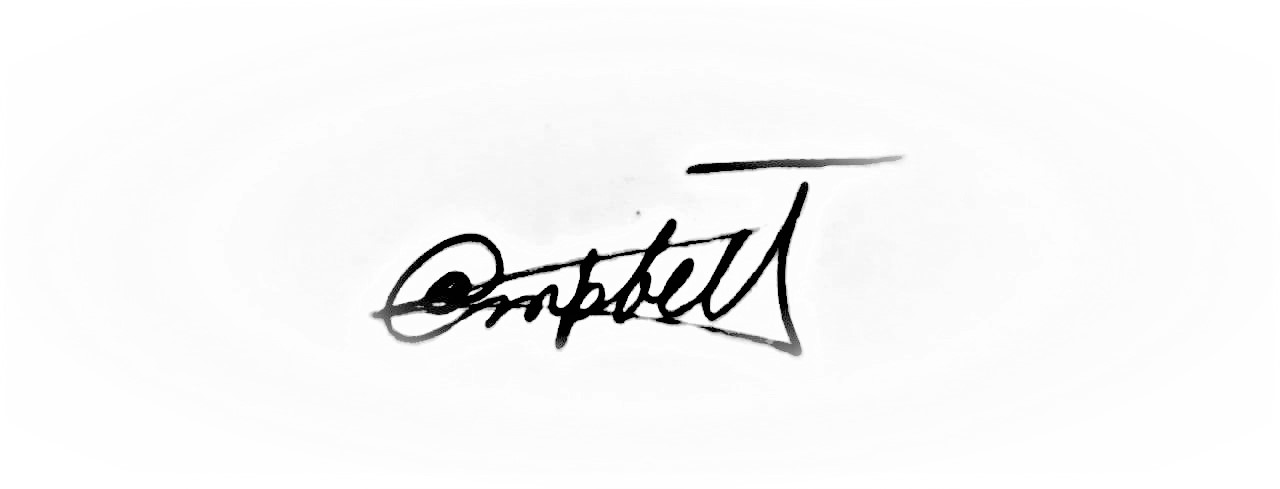
\includegraphics[scale=0.2]{images/firma.jpg}

%% Las secciones del "prefacio" inician con el comando \prefacesection{T'itulo}
%% Este tipo de secciones *no* van numeradas, pero s'i aparecen en el 'indice.
%%
%% Si quieres agregar una secci'on que no vaya n'umerada y que *tampoco*
%% aparesca en el 'indice, usa entonces el comando \chapter*{T'itulo}
%%
%% Recuerda que aqu'i ya puedes escribir acentos como: 'a, 'e, 'i, etc.
%% La letra n con tilde es: 'n.

\prefacesection{Resumen}
En el presente trabajo de diploma se implementar\'an mejoras y nuevas funcionalidades para el servidor Open Latino, relacionadas con los mapas tem\'aticos y con el manejo de su configuraci\'on. Basados en la investigaci\'on sobre otros sistemas y librer\'ias que usan mapas tem\'aticos, se decidi\'o que lo m\'as conveniente fuera la implementaci\'on de un nuevo tipo de tem\'atico, al que llamaremos mapa tem\'atico por clasificaci\'on de tipos, que es m\'as intuitivo para su utilizaci\'on por parte de los usuarios. Tambi\'en, como parte de este trabajo, se encuentra la creaci\'on de un nuevo pedido que devuelve informaci\'on acerca de los tem\'aticos creados en el sistema. Por \'ultimo, luego de analizar las diferentes interfaces visuales para configuraci\'on de servidores, se lleg\'o a la conclusi\'on de que es necesario una implementaci\'on propia que responda a las necesidades de este servidor en particular, usando poderosos frameworks para este fin, como React.

En los cap\'itulos finales se realizan varias pruebas con el fin de verificar el correcto funcionamiento del servidor y de sus nuevas funcionalidades, brindando las conclusiones a las que se arribaron y se propone el trabajo futuro con Open Latino Server (OLS).\\\\

\section*{Palabras Clave}
Mapa tem\'atico, protocolo WMS, React, interfaz de usuario, ASP .Net Core, sistema, servidor, backend, frontend, framework, servidor de mapas, Sistemas de Informaci\'on Geogr\'afica (SIG), SIG Web


\prefacesection{Abstract}
This diploma project is proposed to implement improvements and new functionalities for the Open Latino server, related to the thematic maps and managing server configuration. Based on research on other systems and libraries that use thematic maps, it was decided that the most convenient solution to the problem would be the implementation of a new type of thematic, which we will call thematic map by type classification, which is more intuitive for users. Also, as part of this work, the creation of a new request that returns information about the thematics that are created in the system. Finally, after analyzing the different settings visual interfaces of servers, it was reached the conclusion of an own implementation, that responds to the needs of this server in particular, is necessary, using powerful frameworks, like React. 

Several tests are performed in the final chapters to verify the correct operation of the server and its new functionalities, providing the conclusions that we arrived and future work with Open Latino Server(OLS).\\\\

\section*{KeyWords}
Thematic map, WMS protocol, React, user interface, ASP .Net Core, system, server, backend, frontend, framework, Internet Map Server (IMS), Geografic Information System (GIS), Web GIS

\tableofcontents
\listoffigures
%\listoftables

%% # Cap'itulos #
%% Por cada cap'itulo hay que crear un nuevo archivo e incluirlo aqu'i.
%% Mirar el archivo "intro.tex" para un ejemplo y recomendaciones para
%% escribir.

%% Los cap'itulos inician con \chapter{T'itulo}, estos aparecen numerados y
%% se incluyen en el 'indice general.
%%
%% Recuerda que aqu'i ya puedes escribir acentos como: 'a, 'e, 'i, etc.
%% La letra n con tilde es: 'n.

\chapter{Introducci\'on}

Hasta hace algunas d\'ecadas, los mapas se realizaban obteniendo las coordenadas de los puntos por m\'etodos geod\'esicos, topogr\'aficos y astron\'omicos para que despu\'es mediante m\'etodos cartogr\'aficos se elaborara el mapa correspondiente de acuerdo con la proyecci\'on y la escala seleccionada; sin embargo, a partir de la d\'ecada de los 70, con el lanzamiento de los sat\'elites Landsat y con el establecimientos de los procesos cartogr\'aficos digitales, la forma de hacer mapas paulatinamente se volvi\'o m\'as din\'amica. En la actualidad, usando los diferentes sat\'elites, GPS \footnote{Sistema de navegaci\'on y localizaci\'on mediante sat\'elites.} y los Sistemas de Informaci\'on Geogr\'afica (SIG) \footnote{Sistema de informaci\'on capaz de integrar, almacenar, editar, analizar, compartir y mostrar la informaci\'on geogr\'aficamente referenciada.}, el ser humano elabora diferentes mapas que permiten analizar con mayor profundidad la informaci\'on contenida en un territorio.

Un mapa es la representaci\'on gr\'afica de un territorio sobre una superficie bidimensional. Se define tambi\'en como un dibujo o trazado esquem\'atico que representa las caracter\'isticas de un territorio determinado, tales como sus dimensiones, coordenadas, accidentes geogr\'aficos u otros aspectos relevantes. La funci\'on principal de los mapas es brindar
informaci\'on sintetizada sobre puntos de localizaci\'on y coordenadas de orientaci\'on, as\'i como tambi\'en sobre rutas disponibles, caracter\'isticas de la superficie terrestre (relieves, redes fluviales, recursos, etc.), clima regional, l\'imites pol\'itico-territoriales, puntos de inter\'es, distribuci\'on de la poblaci\'on, etc.\cite{mapa}

El siglo XX fue testigo de un avance extraordinario en el desarrollo de la cartograf\'ia, decisivo en este sentido fue el desarrollo de la fotograf\'ia a\'erea y el despliegue satelital hasta llegar al uso de Sistemas de Informaci\'on Geogr\'afica \cite{SIG} (SIG o GIS, por sus siglas en ingl\'es, Geografic Information System).

En las \'ultimas cinco d\'ecadas, los Sistemas de Informaci\'on Geogr\'afica han evolucionado desde un concepto a una ciencia. Esta magn\'ifica evoluci\'on hace que los SIG pasen de ser una herramienta rudimentaria a convertirse en una poderosa
plataforma para comprender y planificar nuestro mundo. El campo de los Sistemas de Informaci\'on Geogr\'afica est\'a marcado por diversos hitos, comenz\'o en los a\~nos sesenta, mientras emerg\'ian las computadoras y los primeros conceptos de geograf\'ia cuantitativa y computacional. El trabajo pionero de Roger Tomlinson \cite{robert} para iniciar, planificar y desarrollar el Sistema de Informaci\'on Geogr\'afica de Canad\'a, dio como resultado el primer SIG computarizado del mundo, en 1963.

El futuro de SIG, junto con su pasaje a la web y computaci\'on en la nube y la integraci\'on con la informaci\'on en tiempo real a trav\'es del internet de las cosas(IoT) \footnote{es el proceso que permite conectar elementos f\'isicos cotidianos al Internet \cite{iot}}, se convirti\'o en una plataforma relevante a casi toda actividad humana, el sistema nervioso del planeta. Mientras que el mundo enfrenta desaf\'ios, tales como la expansi\'on de la poblaci\'on, desforestaci\'on y contaminaci\'on, los SIG \cite{FSIG} jugar\'an un papel cada vez m\'as importante en c\'omo entendemos y abordamos estos problemas y proporcionan el medio para comunicar soluciones utilizando el lenguaje com\'un de los mapas.

El acelerado desarrollo de internet hizo m\'as f\'acil compartir y actualizar la informaci\'on, lo que motiv\'o el surgimiento de los Web GIS, un patr\'on para la implementaci\'on de un GIS moderno, impulsado por un web-servicio estandar que entrega
datos, capacidades y conecta componentes. Un Web GIS puede ser implementado en la nube con permisos o, m\'as com\'un, como una combinaci\'on h\'ibrida obteniendo lo mejor de ambos mundos. Dentro de sus componentes m\'as importantes se encuentra el Servidor de Mapas(en ingl\'es conocido como IMS: Internet Map Server) \cite{webGis}, de gran utilidad para manejar grandes vol\'umenes de informaci\'on provenientes de diversos proveedores y realizar diversas consultas u operaciones (Queries en ingl\'es) sobre los datos que maneja en solo unos milisegundos, incluso si se trata de millones de datos.

A ra\'iz de estos avances tecnol\'ogicos, surgieron nuevas herramientas que facilitan el estudio cient\'ifico a partir de variables diversas y complejas; como ejemplo, se pueden mencionar los mapas de edificios en una ciudad que constituyan hospitales. Su diferencia radica principalmente en la escala del mapa; es decir, generales o detallados, dependiendo del nivel de especializaci\'on al que desee alcanzar el investigador. Esto no es m\'as que un mapa tem\'atico.

Una de las funcionalidades que tambi\'en tienen los IMS es la de dar, precisamente, mapas tem\'aticos, cuyo objetivo es reflejar un aspecto particular de la zona geogr\'afica sobre la que se definen. Pueden centrarse en variables f\'isicas, sociales, pol\'iticas, culturales, econ\'omicas, sociol\'ogicas y cualquier otra relacionada con un territorio concreto. Los mapas tem\'aticos recogen y aportan informaci\'on sobre temas geogr\'aficos peculiares. Pueden ser anal\'iticos si representan un \'unico elemento gr\'afico, o sint\'eticos si re\'unen datos de diferentes mapas. \cite{tematico}

Una diferenciaci\'on necesaria los clasifica en cualitativos (aquellos que representan fen\'omenos sin tener ninguna precisi\'on num\'erica) y cuantitativos (los que representan el valor num\'erico de un fen\'omeno). As\'i pues, nos encontramos ante una gran
variedad de tipos de mapas tem\'aticos. Entre ellos, destacan los de isol\'ineas, que usan l\'ineas curvas para unir puntos de igual valor de un fen\'omeno, los mapas de flujos, que consisten en l\'ineas de diferente espesor para representaciones din\'amicas y los mapas anam\'orficos, que dependen de la magnitud del fen\'omeno representado \cite{tematico}. Es decir, cambian el tama\~no real de los pa\'ises para hacerlo proporcional al hecho que cartograf\'ian. Los mapas tem\'aticos utilizan los mapas topogr\'aficos \footnote{una imagen, generalmente del relieve de la superficie terrestre, a una escala definida.} como mapas base para la representaci\'on gr\'afica de datos de diversa \'indole, lo que se conoce como cartograf\'ia tem\'atica.

Los servidores de mapas son los encargados de servir los Datos Espaciales \footnote{dato que tiene asociada una referencia geogr\'afica de tal modo que se puede localizar exactamente d\'onde sucede dentro de un mapa.} de los territorios, los cuales son agrupados en conjuntos, denominados Capas, que al combinarse dan como resultado los mapas, adem\'as si se le agregan a estas capas un grupo de restricciones se obtiene un mapa tem\'atico \cite{MP}. Estas capas pueden contener
dos tipos de datos: Raster que son cualquier tipo de imagen digital representada en mallas o Vectorial que est\'an destinados a almacenar con gran exactitud los elementos geogr\'aficos. Cada uno de estos est\'a vinculado a una fila en una base de datos que
describe sus atributos y pol\'igonos.

El desarrollo exponencial, a pasos acelerados, de la humanidad y su relaci\'on directa con el perfeccionamiento de los SIG constituyen la raz\'on de ser de esta investigaci\'on, con \'enfasis en los mapas tem\'aticos, haci\'endolos m\'as \'utiles y f\'aciles de manejar por los usuarios, llev\'andolos a un nivel superior, donde se haga m\'as simple su manejo pero a la vez m\'as complejo y espec\'ifico su contenido, mejorando su eficacia.



\section{Formulaci\'on del problema, motivaci\'on y justificaci\'on}

La Casa del Software de la Facultad de Matem\'atica y Computaci\'on de la Universidad de La Habana ha venido desarrollando un Sistema de Informaci\'on Geogr\'afica llamado Open Latino GIS. Entre los componentes de este sistema se encuentra Open Latino Server (OLS). Este servidor fue desarrollado usando las buenas pr\'acticas de la programaci\'on orientada a objetos \cite{OO} y los principios SOLID \cite{solid} por lo que su c\'odigo es f\'acil de entender y permite incorporar mejoras f\'acilmente. Fue creado usando la tecnolog\'ia de ASP.NET Framework \cite{aspnet}, en consecuencia, solo pod\'ia ejecutarse en entorno Windows y publicarse usando IIS \cite{iis}.

Teniendo como objetivo que fuera multiplataforma \footnote{proyectos que operan en m\'ultiples plataformas inform\'aticas.}, se desarroll\'o una versi\'on 2.0 utilizando NET CORE \cite{netcore}. La nueva versi\'on de OLS complet\'o la implementaci\'on del protocolo WMS \footnote{El protocolo est\'andar WMS permite, a grandes rasgos, servir im\'agenes georeferenciadas a trav\'es de internet} (Web Map Service) \cite{wms} que se encontraba pendiente en su versi\'on anterior. En este se encuentran una serie de pedidos b\'asicos entre los que se puede destacar GetMap, GetCapabilities,etc. Este servidor cuenta, adem\'as, con un pedido para visualizar mapas tem\'aticos.

A pesar de las muchas funcionalidades con las que se cuenta, se presenta el problema de que este servidor carece de una interfaz de usuario\footnote{Punto de interacci\'on y comunicaci\'on humano-computadora en un dispositivo.} amigable, para poder configurarlo es necesario hacerlo a nivel de c\'odigo, mediante el uso de programas para modificar las bases de datos. OLS tampoco cuenta con una funcionalidad que permita conocer los detalles acerca de los tem\'aticos que est\'an definidos en este, actualmente se deben realizar consultas sql \footnote{Structured Query Language, lenguaje de programaci\'on que te permite manipular y descargar datos de una base de datos} para conocer esa informaci\'on. Por \'ultimo, los tem\'aticos que existen son por consulta, es decir, la definici\'on de nuevos tem\'aticos se realiza usando consultas de sql.

Resulta de importancia agregar las funcionalidades anteriores al servidor ya que al usuario final se le dificulta el trabajo con el sistema, debido a que debe tener nociones elementales de programaci\'on y conociminetos b\'asicos de sql para manipular la configuraci\'on de OLS e interactuar con las funcionalidades referentes a los mapas tem\'aticos. Se hace necesario, entonces, la implementaci\'on de una interfaz de usuario amigable para el trabajo con la configuraci\'on del servidor y los mapas tem\'aticos, as\'i como el desarrollo de un nuevo tipo de mapas tem\'aticos, m\'as intuitivo, de clasificaci\'on por tipos. Adem\'as, de la creaci\'on de un nuevo pedido que devuelva toda la informaci\'on relacionada a los tem\'aticos definidos en OLS.

Para dar soluci\'on a las cuestiones planteadas anteriormente, es necesario dar respuesta a las siguientes preguntas:

\begin{itemize}
\item ?`Existen en la actualidad soluciones que permitan representar la informaci\'on estad\'istica con la que cuentan las personas en un \'area geoespacial determinada?
\item ?`Existen soluciones para la representaci\'on de la informaci\'on estad\'istica que poseen los usuarios sobre el espacio geogr\'afico de su inter\'es que sea capaz de integrar disponibilidad, accesibilidad y robustez, para que los usuarios cuenten
con un mecanismo eficiente que les apoye en la formaci\'on de elementos de juicio para la toma de decisiones?
\item ?`Es posible crear un software que sea de c\'odigo abierto y que adem\'as est\'e disponible estando en l\'inea, que tenga una herramienta para brindar visualizaci\'on sobre el problema en cuesti\'on?
\item ?`Qu\'e soluciones y tecnolog\'ias existentes son apropiadas para la implementaci\'on de la presente investigaci\'on?
\end{itemize}

Es posible dar soluci\'on a las preguntas anteriores gracias a los conocimientos, herramientas y habilidades de investigaci\'on adquiridas en el transcurso de los estudios universitarios en la carrera de Ciencias de la Computaci\'on de la Universidad de La Habana. Se cuenta, adem\'as, con las tecnolog\'ias necesarias, ya se han puesto en uso en la plataforma OLS que se presta como antecedente a los nuevos cambios propuestos, adem\'as se cuenta con aplicaciones precedentes en el propio Departamento de Programaci\'on, Ingenier\'ia de Software y Base de Datos como son C-sharp, ASP.Net Core, SQL Server entre otras que evidencian una rica experiencia de base.


\section{Objetivos}
Para resolver el problema anunciado anteriormente se plantean los siguientes objetivos principales:

\begin{enumerate}
\item Desarrollar una herramienta sobre la plataforma de c\'odigo abierto OLS que presente un mecanismo para visualizar y configurar un nuevo tipo de mapas tem\'aticos clasificados por valores de forma extensible.
\item Implementar una herramienta que permita consultar informaci\'on acerca de los tem\'aticos existentes en el servidor.
\item Desarrollar una interfaz visual intuitiva para manipular la configuraci\'on del servidor y los mapas tem\'aticos.
\end{enumerate}

Para cumplir con los objetivos principales explicados previamente, se plantean los siguientes objetivos secundarios:

\begin{enumerate}
\item Estudiar precedentes de otras aplicaciones que tengan implementado una herramienta para visualizar y configurar mapas tem\'aticos.
\item Investigar las ventajas, desventajas y analizar la factibilidad de las mejores herramientas para implementar la interfaz visual.
\item Extender la arquitectura de clases con la que ya cuenta OLS que cumpla con los principios del SOLID, que sea extensible y mantenible para continuar con las buenas pr\'acticas de la plataforma OLS para que cualquier implementaci\'on posterior en este tema se pueda utilizar sin necesidad de modificar, aumentando la eficacia y sencillez de futuras mejoras al proyecto.
\end{enumerate}


\section{Estructura del trabajo}
Este trabajo de diploma est\'a compuesto por 5 cap\'itulos y se estructura de la siguiente manera:

\begin{itemize}
\item \textbf {Cap\'itulo 1 :} \qquad El primer cap\'itulo presenta una breve introducci\'on al tema, la motivaci\'on, formulaci\'on del problema y justificaci\'on del mismo, los objetivos principales y secundarios, concluyendo este cap\'itulo con la estructura del trabajo de diploma.
\item \textbf {Cap\'itulo 2 :} \qquad Este cap\'itulo est\'a dedicado al estado del arte, donde se analizar\'an del uso de los diferentes IMS que implementan los mapas tem\'aticos por clasificaci\'on, as\'i como de las diferentes interfaces visuales que existen para configurar un servidor. Se expondr\'an las ventajas y desventajas de su uso.
\item \textbf {Cap\'itulo 3 :} \qquad En este cap\'itulo se expone el marco te\'orico-conceptual del presente trabajo, donde se explican las soluciones que se dieron a los objetivos, tanto conceptualmente como algunos de sus detalles de implementaci\'on. Adem\'as, se aborda acerca del mecanismo que se implementa para la recuperaci\'on de tem\'aticos y la integraci\'on del nuevo tipo de mapa, as\'i como se expondr\'a la arquitectura usada en la implementaci\'on de la interfaz visual. Por \'ultimo se da una explicaci\'on de las tecnolog\'ias empleadas y d\'onde se usaron.
\item \textbf {Cap\'itulo 4 :} \qquad El cap\'itulo 4 est\'a dedicado a exponer un conjunto de pruebas para mostrar el buen funcionamiento de la nueva versi\'on de OLS y el cumplimineto de los objetivos planteados. En estas pruebas se van planteando los objetivos que se quieren verificar con estas y luego se presentan los resultados alcanzados con cada una.
\item \textbf {Cap\'itulo 5 :} \qquad En el quinto y \'ultimo cap\'itulo se proponen las conclusiones y recomendaciones, temas para trabajo futuro, es decir, temas que quedaron pendientes o se pueden realizar de una mejor manera. En este cap\'itulo aparece, adem\'as, la bibliograf\'ia utilizada.
\end{itemize}



%% Los cap'itulos inician con \chapter{T'itulo}, estos aparecen numerados y
%% se incluyen en el 'indice general.
%%
%% Recuerda que aqu'i ya puedes escribir acentos como: 'a, 'e, 'i, etc.
%% La letra n con tilde es: 'n.

\chapter{Estado del Arte}

A lo largo de este cap\'itulo se explica el punto m\'as avanzado en que se encuentra hoy en d\'ia los SIG y los servidores de mapas, haciendo incapi\'e en aquellos que implementan mapas tem\'aticos, sin pasar por alto la interfaz de usuario que utilizan para la configuraci\'on de servidor. Por \'ultimo, basado en la investigaci\'on de las herramientas existentes que utilizan mapas tem\'aticos y de la interfaz visual para su configuraci\'on, se decide la mejor estrategia para utilizar sobre el servidor. No sin antes acercar al lector a la historia del origen y evoluci\'on de los mapas tem\'aticos.


\section{Origen y evoluci\'on de los mapas tem\'aticos}

Claudio Tolomeo (siglo II), griego o egipcio, es mejor conocido como el astr\'onomo autor de la idea err\'onea del Universo, sostenida durante catorce siglos, seg\'un la cual la Tierra ocupa el centro y los planetas giran a su alrededor. Sin embargo, el gran m\'erito de Tolomeo radica en la geograf\'ia.

Los mapas tem\'aticos tienen su antecedente en Tolomeo, quien los elabor\'o de tipo hist\'orico. En forma aislada aparecieron desde el siglo XVIII mapas espec\'ificos para representar alg\'un fen\'omeno de la naturaleza, adem\'as de los hist\'oricos que fueron los m\'as comunes. En la segunda mitad de este siglo se popularizaron los t\'erminos mapa y cartograf\'ia tem\'aticos y, en esta \'epoca, se han multiplicado en grado superlativo. Los primeros mapas tem\'aticos fueron muy simples, sin embargo, ameritaron su publicaci\'on en las revistas geol\'ogicas de mayor prestigio, aunque presentaban una informaci\'on muy general y pobre en extremo, nadie puede negar el inmenso valor de esa informaci\'on.\cite{histTematico}

Si los mapas alcanzan un grado, digamos cercano a la perfecci\'on, puede pensarse que el tema de investigaci\'on queda clausurado. Esto es cierto s\'olo parcialmente. En la medida que los mapas que representaban rasgos f\'isicos de la superficie terrestre se fueron perfeccionando, surgi\'o la necesidad de expresar otros fen\'omenos y objetos: los suelos, las comunidades de flora y fauna, las rocas, los climas, la estructura profunda de la Tierra. De la cartograf\'ia general se pas\'o a la tem\'atica.

El mapa ha sido siempre un reflejo del estado de desarrollo de determinadas disciplinas cient\'ificas. Si actualmente hay decenas o cientos de mapas tem\'aticos diversos, esto da una idea del estado actual de las geociencias. Uno de los m\'as conocidos es el publicado en 1936 sobre la agricultura de Estados Unidos. Destac\'o por su originalidad. Posteriormente han sido editados mapas complejos en diversos pa\'ises, resultado de investigaciones prolongadas e incluso multidisciplinarias, apoyadas por instituciones cient\'ificas y financieras.

Los mapas tem\'aticos de un mismo pa\'is o regi\'on se hacen peri\'odicamente, pretenden que la informaci\'on contenida en el mismo sea f\'acilmente comprendida por el lector o usuario. Si esta es correcta y valiosa, pero mal expresada por no usar los colores o s\'imbolos adecuados, la lectura del mapa se vuelve labor tortuosa. Por esto, el dise\~no final queda a cargo de un especialista altamente calificado, quien define colores, s\'imbolos, tama\~nos de letras, grosor de l\'ineas, distribuci\'on de la leyenda y otros problemas semejantes. Es la parte art\'istica de la cartograf\'ia. \cite{histTematico}

En los \'ultimos quince a\~nos asistimos a una aut\'entica revoluci\'on en el amplio campo de la cartograf\'ia, y muy especialmente en la caracterizaci\'on tridimensional del territorio. Se ha pasado en unas d\'ecadas de una cartograf\'ia casi secreta, en manos de los ej\'ercitos o de los estados, y muy limitada, a una enorme disponibilidad e incluso a la gratuidad de los materiales. Con el tiempo se han creado servidores que facilitan cartograf\'ia tem\'atica a cualquier usuario. Los servidores permiten visualizar mapas, la localizaci\'on, la identificaci\'on de atributos, las consultas sencillas e incluso la conexi\'on a bases de datos remotas para poder crear mapas tem\'aticos. \cite{sigTematico}



\section{Herramientas SIG que implementan mapas tem\'aticos}

Hoy en d\'ia existen servicios en l\'inea que son capaces de generar mapas tem\'aticos a partir de ciertos par\'ametros de entrada. Sin embargo es peque\~na la cantidad de t\'ecnicas de representaci\'on de datos estad\'isticos que se pueden manejar, en general los datos estad\'isticos y geogr\'aficos disponibles son los que se encuentran en los servidores de quienes administran el servicio y, en la mayor\'ia de los casos, su c\'odigo no puede ser descargado ni modificado de acuerdo a las necesidades de los usuarios. Existen herramientas de escritorio y, adem\'as, plataformas que usan servidores de mapas, lo cuales cuentan con m\'odulos que permiten la creaci\'on de mapas tem\'aticos y dejan al usuario utilizar los datos estad\'isticos que posee, sin embargo, estas son aplicaciones que no se centran en el trabajo con mapas tem\'aticos, sino en la edici\'on y gesti\'on de datos geogr\'aficos por lo que en su mayor\'ia el n\'umero de t\'ecnicas de representaci\'on de datos estad\'isticos con el que se trabaja no es muy amplio; adem\'as, en no todos los casos el c\'odigo fuente est\'a disponible.


\subsection{QGis}
QGis es un sistema de informaci\'on geogr\'afica de software libre\footnote{significa que los usuarios tienen la libertad de ejecutar, copiar, distribuir, estudiar, modificar y mejorar el software} y de c\'odigo abierto\footnote{software cuyo c\'odigo fuente se ha puesto a disposici\'on de todo el mundo de manera gratuita}, multiplataforma, que funciona junto con un servidor web \cite{ART}. Esta herramienta cuenta con un peque\~no m\'odulo para crear mapas tem\'aticos. La ayuda del software hace una descripci\'on acerca del uso de los mismos, en esta se plantea que est\'an disponibles cuatro modos para crear diferentes tipos de estos mapas.  

Como ventajas, este sistema multiplataforma de c\'odigo abierto presenta funcionalidades para la creaci\'on de los mapas tem\'aticos, que permiten seleccionar, en un men\'u deplegable, varias opciones; la que nos concierne es la de Categorized, que permite asignar un color diferente a cada capa, y as\'i, crear un mapa tem\'atico, donde separa por colores la informaci\'on pertinente a estas. Adem\'as, una de las mayores ventajas de esta herramienta es la posibilidad de usar Quantum GIS como GUI (Interfaz gr\'afica de usuario) del SIG GRASS \cite{qgis}, utilizando toda la potencia de an\'alisis de este \'ultimo en un entorno de trabajo m\'as amigable. QGIS est\'a desarrollado en C++\footnote{lenguaje de programaci\'on multiparadigma dise\~nado en 1979 por Bjarne Stroustrup.}, usando la biblioteca Qt\footnote{framework multiplataforma orientado a objetos ampliamente usado para desarrollar programas que utilicen interfaz gr\'afica de usuario} para su Interfaz gr\'afica de usuario.

A pesar de las ventajas expuestas, QGis presenta varias desventajas, que no perminten su uso en Open Latino Sever. Entre estas se encuentran que no son muchos los tipos de mapas tem\'aticos que pueden ser creados utilizando QGis. Tampoco se puede integrar al proyecto OLS con facilidad debido a que est\'a en otro lenguaje y, para a\~nadirlo, habr\'ia que migrar todo el c\'odigo a C-sharp, que ser\'ia tan o m\'as costoso que implementar la herramienta de mapas tem\'aticos desde cero, adem\'as, esto no garantizar\'a que la migraci\'on quede libre de errores. Tambi\'en se puede decir que esta herramienta no permite realizar restricciones sobre una misma capa para tematizar la informaci\'on de esta. Por \'ultimo, a pesar de que existen bindings de la librer\'ia Qt de interfaz de usuario para C-sharp, se dificulta su uso por la misma problem\'atica de la migraci\'on de c\'odigo, sin dejar de mencionar que es necesario modificar, por no decir, cambiar por completo el c\'odigo de la interfaz, puesto que el manejo de la configuraci\'on de QGis se diferencia, en gran medida, con la de OLS, osea que no podemos integrar directamente el frontend al servidor, sino que se tiene que adaptar, en cuyo caso es preferible hacer una interfaz propia con un framework que se ajuste a las necesidades de OLS.


\subsection{ArcGis}
ArcGis es un completo sistema que permite recopilar, organizar, administrar, analizar, compartir y distribuir informaci\'on geogr\'afica. Permite crear y utilizar Sistemas de Informaci\'on Geogr\'afica. Una de las principales funcionalidades de ArcGIS es la creaci\'on y dise\~no de cartograf\'ia. Los mapas generados pueden ser de diversa tipolog\'ia, siendo una de las m\'as destacadas la de mapas tem\'aticos. Estos mapas permiten captar el inter\'es de los usuarios y proporcionarles informaci\'on de forma muy visual, ofreciendo un m\'etodo ideal para mostrar los resultados del trabajo SIG.

Las ventajas que presenta esta herramienta radican en que proporciona una amplia posibilidad de recursos relacionados con los mapas tem\'aticos. Con esta herramienta se pueden crear, consultar y analizar datos; combinar varias capas; aplicar funciones matem\'aticas, construir y obtener nueva informaci\'on a partir de tem\'aticos ya existentes, etc. En ArcGis, la finalidad de un mapa tem\'atico es la de representar de una o varias caracter\'isticas de fen\'omenos geogr\'aficos, pudiendo dividir a estos en objetos reales: distribuci\'on, densidad, relaci\'on, etc; y conceptos abstractos: indicadores de desarrollo econ\'omico, calidad de vida, etc. Estos mapas pueden ser publicados en web permitiendo, mediante ventanas emergentes, la visualizaci\'on de una o varias de estas caracter\'isticas,  fotograf\'ias de los fen\'omenos y acceso a otra informaci\'on en la web. \cite{ART}

La principal desventaja que presenta este software es que no es c\'odigo abierto, sino que se distribuye comercialmente bajo tres niveles de licencia, por lo tanto se descarta por no ser de c\'odigo abierto y no ser gratuito. Adem\'as, la interfaz de usuario que presenta es un poco complicada, debido a que cada documento diferente en ArcGIS utiliza una GUI separada, cada GUI se compone por barra de botones, herramientas, men\'us, estados y l\'ineas de comando, lo que dificulta su uso por usuarios poco preparados, y no es lo que se quiere en OLS.


\subsection{MapInfo}
Las soluciones que proporciona MapInfo \cite{mapinfo} para la creaci\'on de mapas permiten llevar a cabo an\'alisis geogr\'aficos sencillos y complejos, acceso a datos remotos y creaci\'on de mapas tem\'aticos que revelen patrones en los datos. Se pueden visualizar los datos como puntos, regiones zonificadas tem\'aticamente, como gr\'aficos de tartas o de barras , etc.

Como parte de las caracter\'isticas ventajosas se encuentran que, con MapInfo, se pueden crear distintos mapas tem\'aticos asign\'andoles a estos colores, patrones o s\'imbolos para establecer una coincidencia con objetos seg\'un valores espec\'ificos de la tabla. La caracter\'istica Mapa tem\'atico utiliza un asistente compuesto de una secuencia de tres cuadros de di\'alogo que facilitan la selecci\'on del tipo de mapa tem\'atico que se desea, las tablas y los campos que se utilizar\'an para construir el mapa y diversas opciones para personalizarlo. Las plantillas tem\'aticas de MapInfo facilitan el comienzo de la creaci\'on de un tema. Se selecciona una plantilla que represente el tipo de mapa tem\'atico que se desea. Las plantillas se pueden personalizar completamente y pueden guardarse como nuevas plantillas en caso de que se precisen para la creaci\'on de mapas tem\'aticos m\'as adelante. Con MapInfo se suministran m\'as de 40 plantillas. MapInfo cuenta con una potente y flexible interfaz de usuario, interactiva para mapas tem\'aticos, esta interfaz permite a los usuarios anclar las barras de herramientas en los cuatro lados de la aplicaci\'on, ayudando a mejorar la eficiencia, reducir la conglomeraci\'on sobre la pantalla, y ahorrar tiempo. \cite{mapinfo}

Como parte de las desventajas que nos inclinan a descartar a MapInfo se encuentra que no es multiplataforma, solo est\'a disponible para Windows\footnote{sistema operativo, es decir, un conjunto de programas que posibilita la administraci\'on de los recursos de una computadora}. Adem\'as, es un software privado de la compa\~n\'ia Precisely, antiguamente Pitney Bowes Inc, lo que no se corresponde con las pol\'iticas de migraci\'on a software libre e imposibilita su adquisici\'on. Finalmente, es un software basado en Python\footnote{lenguaje de programaci\'on ampliamente utilizado en las aplicaciones web, el desarrollo de software, la ciencia de datos y el machine learning}, lo cual entorpecer\'ia su integraci\'on a OLS por la problem\'atica antes mencionada de migraci\'on de c\'odigo.


\subsection{SharpMap}
SharpMap \cite{sharpmap} es una biblioteca de clases para crear aplicaciones web. Con esta librer\'ia se pueden realizar consultas a los datos espaciales para el manejo y an\'alisis de los mismos.

Ser\'ia ventajoso el uso de SharMap ya que es un sistema SIG escrito totalmente en C\# .NET 4.0, y admite m\'ultiples lenguajes de desarrollo .Net (C\#, C$++$, etc). Tambi\'en, presenta la clase \textit{CustomTheme}, que es usada para definir un tem\'atico propio, esta presenta dos m\'etodos p\'ublicos: \textit{CustomTheme}, para crear la clase, y \textit{GetStyle}, para obtener un estilo para pintar el tem\'atico. Adem\'as, con la herramienta \textit{SharpMap.Rendering.Thematics.CategoryTheme} se crean categor\'ias usando rangos de valores para comparar con el campo elegido. \cite{sharpmap}

Una notale desventaja de esta biblioteca es que al no ser multiplataforma dar\'ia un paso atr\'as en el desarrollo de OLS, que ya
fue mejorado a un proyecto multiplataforma. Por otro lado, al estar basado en el framework .Net 4.0, y este no presentar una versi\'on compatible con ASP.NET Core, entra en conflicto con la \'ultima versi\'on de OLS, que ya fue migrado a ASP.NET Core. SharpMap carece, adem\'as, de una interfaz visual, por lo que es necesario usar c\'odigo, lo cual dificulta a usuarios que no est\'en familiarizados con la programaci\'on hacer uso de esta, y es una de las cosas que se quiere evitar en OLS. Por \'ultimo, otra restricci\'on que presenta esta biblioteca, es que no presenta muchos tipos de tem\'aticos.


\section{Frameworks y librer\'ias de JavaScript que se pueden utilizar en la interfaz visual de OLS.}

Como se dijo anteriormente, se hace necesario la creaci\'on de una interfaz propia que responda a las necesidades particulares de OLS. Los Frameworks de interfaz gr\'afica son soluciones completas que contemplan herramientas de apoyo a la construcci\'on de software para la capa de presentaci\'on, brindando al usuario aplicaciones atractivas. Las bibliotecas, y los marcos de trabajo de JavaScript\footnote{lenguaje de programaci\'on que se utiliza para hacer p\'aginas web interactivas}, facilitan el desarrollo de sitios web y aplicaciones con caracter\'isticas y funcionalidades muy variadas, todo ello gracias a las caracter\'isticas din\'amicas, flexibles y atractivas de JavaScript. Seg\'un una encuesta de StackOverflow\footnote{sitio de preguntas y respuestas para desarrolladores dise\~nado para resolver problemas y aprender} de 2020, JavaScript sigue siendo el lenguaje de programaci\'on m\'as utilizado (por octavo a\~no), con un 67,7\% de los encuestados que lo utilizan. Su versatilidad favorece el desarrollo del front-end, adem\'as de las pruebas. Como resultado, se pueden encontrar muchas bibliotecas y frameworks de JavaScript que sirven para varios prop\'ositos. En el mercado existe una amplia gama de Frameworks y librer\'ias que proveen soluciones para el desarrollo de aplicaciones web, y la creaci\'on de interfaces gr\'aficas. En este ep\'igrafe se estudiar\'an aquellos que, por sus caracter\'isticas y su uso en el mundo de la programaci\'on web, se consideran m\'as importantes.


\subsection{React}
ReactJS es una librer\'ia escrita en JavaScript de c\'odigo abierto enfocada a la visualizaci\'on para facilitar la creaci\'on de componentes interactivos y reutilizables para interfaces de usuario \cite{react}. Esta librer\'ia fue lanzada en el a\~no 2013 y desarrollada por Facebook, quienes tambi\'en la mantienen actualmente junto a una comunidad de desarrolladores independientes y compa\~n\'ias. La caracter\'istica m\'as importante de ReactJS es el componente, una pieza de interfaz de usuario. Al dise\~nar una App con React, lo que se crean son componentes independientes y reusables para crear interfaces de usuario m\'as complejas. De esta manera, ReactJS est\'a basado en un paradigma llamado programaci\'on orientada a componentes en el que cada componente es una pieza con la que el usuario puede interactuar. Estas piezas se crean usando una sintaxis llamada JSX \cite{react} permitiendo escribir HTML\footnote{lenguaje con el que se define el contenido de las p\'aginas web} (y opcionalmente CSS\footnote{lenguaje que maneja el dise\~no y presentaci\'on de las p\'aginas web}) dentro de objetos JavaScript.

Entre las muchas ventajas que tiene el uso de React resalta el desarrollo rentable, ofreciendo una v\'ia econ\'omica para crear aplicaciones multiplataforma. Adem\'as, se necesitan menos esfuerzos, ya que se requiere menos c\'odigo en comparaci\'on con otras plataformas de desarrollo. Tambi\'en, dado el hecho de que ReactJS es una plataforma de c\'odigo abierto con licencia del MIT, brinda acceso para usar bibliotecas y marcos de forma gratuita.

Como parte de las desventajas que motivaron a no usar esta biblioteca se destacan la ausencia de documentaci\'on oficial. La alta velocidad de desarrollo de ReactJS apenas deja lugar a una documentaci\'on apropiada, la cual es algo ca\'otica ya que diferentes desarrolladores contribuyen sin un enfoque com\'un. Por otro lado, no existe un est\'andar de desarrollo, de modo que tenemos demasiadas elecciones a tomar. Adem\'as, el alto ritmo de desarrollo de esta herramienta, provoca volver a aprender nuevas formas de hacer las cosas regularmente, cada vez que se realizan nuevos cambios, y resulta dif\'icil para los desarrolladores adoptar todos los cambios con todas las actualizaciones continuas. Por \'ultimo, la integraci\'on de React con un marco MVC\footnote{Modelo Vista Controlador, estilo de arquitectura de software que separa los datos de una aplicaci\'on, la interfaz de usuario, y la l\'ogica de negocio en tres componentes distintos} como nuestro servidor requiere una gran cantidad de configuraci\'on.


\subsection{Vue}
Vue es un marco de trabajo flexible y ligero basado en JavaScript que ofrece potentes herramientas web para desarrollar proyectos web frontales modernistas \cite{vue}. Vue tambi\'en se considera un marco JavaScript flexible y evolutivo, ya que permite realizar cambios en el c\'odigo de una aplicaci\'on sin que ello afecte a ninguna caracter\'istica fundamental, lo que permite crear una interfaz de usuario progresiva. La gran flexibilidad de Vue tambi\'en permite a\~nadir m\'odulos a medida y componentes visuales a la funcionalidad de la aplicaci\'on web.

Como parte de las ventajas de esta herramienta podemos mencionar que presenta HTML empoderado, esto significa que Vue.js tiene muchas similitudes con Angular, y esto puede ayudar a optimizar el manejo de bloques HTML usando diferentes componentes. Por otro lado, tiene una documentaci\'on muy completa, que puede acelerar la curva de aprendizaje para desarrolladores y ahorrar mucho tiempo en el desarrollo de una aplicaci\'on, usando s\'olo conocimientos b\'asicos de HTML y JavaScript. Se puede decir, adem\'as, que este framework se usa para construir tanto aplicaciones de p\'agina \'unica (SPA)\footnote{aplicaciones o sitios web que cargan todos los recursos necesarios para navegar por los sitios web en la primera carga de la p\'agina} o complejas interfaces web de aplicaciones. Tambi\'en, Vue.js puede ocupar cerca de 20KB manteniendo su velocidad y flexibilidad, que permite alcanzar un mejor rendimiento en comparaci\'on con otros frameworks. Finalmente, Vue.js ayuda a construir grandes plantillas reutilizables en poco tiempo de acuerdo con su sencilla estructura.

Como desventaja, Vue.js a\'un tiene poca cuota de mercado comparado con Angular o React, lo que significa que los recursos disponibles de este framework a\'un est\'an en su fase inicial. Por otra parte, su gran flexibilidad puede ser un contratiempo, puesto que, en ocasiones, Vue.js puede tener problemas para integrarse en grandes proyectos y a\'un no hay experiencia acerca de posibles soluciones. La barrera del idioma es un contra de esta herramienta ya que el creador es en realidad chino-estadounidense y apoya mucho a la comunidad de desarrollo china. La mayor\'ia de los usuarios son comunidades de habla no inglesa, que son quiz\'as uno de los mayores problemas con este marco. Predominantemente, la mayor parte de la codificaci\'on est\'a escrita en chino, esto complica el trabajo de los desarrolladores de habla inglesa con Vue.js. Por estas razones se ha desestimado el uso de este framework.


\subsection{Angular}
Angular es una plataforma de desarrollo, construida sobre TypeScript\footnote{lenguaje de programaci\'on construido a un nivel superior de JavaScript, que a\~nade tipados est\'aticos y objetos basados en clases}, un framework basado en componentes para crear aplicaciones web escalables. Es una colecci\'on de bibliotecas bien integradas que cubren una amplia variedad de caracter\'isticas, que incluyen enrutamiento, administraci\'on de formularios, comunicaci\'on cliente-servidor y m\'as \cite{angular}. Angular proporciona un conjunto de herramientas que permiten desarrollar, compilar, probar y actualizar el c\'odigo fuente de la aplicaci\'on. Se ha convertido en una alternativa popular para dise\~nar aplicaciones multiplataforma ya que admite arquitecturas MVC y MVVM\footnote{patr\'on Model-View-ViewModel, ayuda a separar limpiamente la l\'ogica empresarial y de presentaci\'on de una aplicaci\'on de su interfaz de usuario} del lado del cliente, lo que facilita a los desarrolladores la creaci\'on de aplicaciones.

Como ventajas, se puede decir que Angular tiene una estructura basada en componentes lo que hace que estos sean altamente reutilizables, y simplifica el proceso de desarrollo. Angular tiene, adem\'as, una gu\'ia de estilo de documentaci\'on y CLI\footnote{herramienta de l\'inea de comandos que se utiliza para inicializar, desarrollar, estructurar y mantener aplicaciones de Angular}, ambas consistencias de unidad. La codificaci\'on consistente tiene varios beneficios como plantillas o fragmentos predefinidos, f\'acil uso de sitios, etc. Tambi\'en, es compatible con arquitectura MVC, y utiliza la fuente HTML para describir la interfaz de usuario de la aplicaci\'on porque es un lenguaje intuitivo, declarativo y menos complicado. Por \'ultimo, cuando se implementa para proyectos de desarrollo web, Angular se integra sin problemas, ofreciendo un marco inteligente y robusto que ahorra mucho tiempo a los desarrolladores. 

Este framework tambi\'en presenta desventajas, entre las que pueden mencionarse su sintaxis compleja, heredada de la primera versi\'on de Angular. Aunque Angular usa TypeScript, que es menos dif\'icil de aprender. Tambi\'en, pueden aparecer problemas con la migraci\'on de anteriores versiones pero, si se usa en OLS, no ser\'an necesarias estas migraciones.

Seg\'un el an\'alisis de las ventajas y desventajas realizadas en este ep\'igrafe, se decide hacer uso del framework Angular para desarrollar la interfaz visual de configuraci\'on de OLS.


\section{Conclusiones}
A lo largo de este cap\'itulo se analizaron varios Sistemas de Informaci\'on Geogr\'afica que implementan mapas tem\'aticos. Se estudiaron QGis, ArcGis, MapInfo y SharpMap. Los cuales presentan deficiencias si se integran a OLS, entre las causas comunes que llevaron a su desestimaci\'on se encuentran que la mayor\'ia de estas herramientas est\'an en otros lenguajes no compatibles con los del servidor OLS, por lo que ser\'ia igual, o m\'as complicado, su migraci\'on a OLS, que desarrollar una herramienta propia desde cero, la excepci\'on a esta desventaja la presenta SharpMap, pero se descart\'o debido a que no es multiplataforma y su versi\'on de .Net Core no es la misma de OLS, adem\'as de no presentar una interfaz visual. Otras complicaciones que se analizaron fueron la poca capacidad para generar tem\'aticos, como es el caso de QGis, donde, adem\'as, su interfaz visual est\'a implementada en otro lenguaje de programaci\'on. Por otro lado, ArcGis no es de c\'odigo abierto y no es gratuito, y tambi\'en esta herramienta presenta una interfaz de usuario compleja. Finalmente, a pesar de que MapInfo presenta una potente y flexible interfaz de usuario y funcionalidades \'utiles para tem\'aticos, se descarta por no ser multiplataforma y ser un software privado.

Por los motivos antes expuestos, se llega a la conclusi\'on de que la mejor opci\'on es implementar una nueva herramienta que permita configurar y visualizar mapas tem\'aticos de clasificaci\'on de tipos.

En el segundo ep\'igrafe, se analizaron ventajas y desventajas de frameworks y librer\'ias de JavaScript con el objetivo de seleccionar uno para implementar la interfaz visual de OLS. Se analizaron React, Vue y Angular como marcos de trabajo. Se pudo observar que React y Vue no son tan estructurados y definidos como puede ser Angular. React, adem\'as, no cuenta con una fuerte documentaci\'on oficial y necesita mucha configuraci\'on para integrarlo a proyectos como OLS. Vue, a pesar de que est\'a ganando popularidad, no cuenta con un fuerte apoyo de la comunidad de programadores como React o Angular, por otro lado, a pesar de tener una gran documentaci\'on, esta est\'a en su mayor\'ia en chino, lo que dificulta su aprendizaje. Finalmente, debido a que Angular esta basado en TypeScript, su modularidad y jerarqu\'ia de componentes, adem\'as del excelente soporte de la comunidad y de Google, entre otras ventajas previamente expuestas, se decide usar este framework para implementar la interfaz visual de OLS.


%% Los cap'itulos inician con \chapter{T'itulo}, estos aparecen numerados y
%% se incluyen en el 'indice general.
%%
%% Recuerda que aqu'i ya puedes escribir acentos como: 'a, 'e, 'i, etc.
%% La letra n con tilde es: 'n.

\chapter{Soluci\'on Te\'orico-Conceptual-Computacional}

El presente cap\'itulo se enfocar\'a en el marco te\'orico-computacional de la propuesta de soluci\'on, abordando las acciones que pueden realizar los usuarios de OLS y la estructura de la aplicaci\'on, as\'i como la arquitectura y patr\'on de visualizaci\'on empleado. Se explicar\'an, adem\'as, las modificaciones realizadas sobre el c\'odigo fuente del servidor, dando a conocer, finalmente, algunos detalles de implementaci\'on de las nuevas herramientas creadas.

\section{Diagrama de casos de uso en Open Latino Server}
Las funcionalidades de OLS son consumidas por usuarios y aplicaciones cliente. Un usuario representa al humano que accede a la interfaz visual y puede hacer determinados cambios como agregar capas, editar tem\'aticos, crear workspaces, etc\'etera. Un cliente constituye una aplicaci\'on registrada para usar los servicios del servidor de mapas\footnote{Los servicios son los tipos de pedidos que se pueden hacer en OLS, por ejemplo: GetMap, GetCapabilities, entre otros}.


\subsection{Usuarios}
En la aplicaci\'on existen dos roles de usuario: Usuario Regular y Admin. Un Usuario Regular es un usuario que se registra en el sistema, y luego puede ingresar mediante nombre de usuario y contrase\~na, para tener acceso a algunas de las funcionalidades de la aplicaci\'on. Admin es un administrador del sistema, tiene permisos para realizar operaciones CRUD\footnote{acr\'onimo de ¨Crear, Leer, Actualizar y Borrar¨ (del original en ingl\'es: Create, Read, Update and Delete), que se usa para referirse a las funciones b\'asicas en bases de datos o a la capa de persistencia en un software.} sobre las entidades para configurar el servidor. La figura \ref{casos1} representa un diagrama de casos de uso\footnote{Permiten visualizar las interacciones que podr\'ia tener un usuario o un cliente con un sistema.} de las funcionalidades generales que tienen los usuarios en OLS.

Un usuario regular puede realizar las siguientes acciones:

$\bullet$ Registrarse en el sistema.

$\bullet$ Iniciar sesi\'on mendiante nombre de usuario y contrase\~na.

$\bullet$ Registrar sus aplicaciones cliente y crear, editar o eliminar Workspaces para las mismas.



\begin{wrapfigure}{l}{0.5\textwidth} 
\vspace{-20pt} 
\begin{center} 
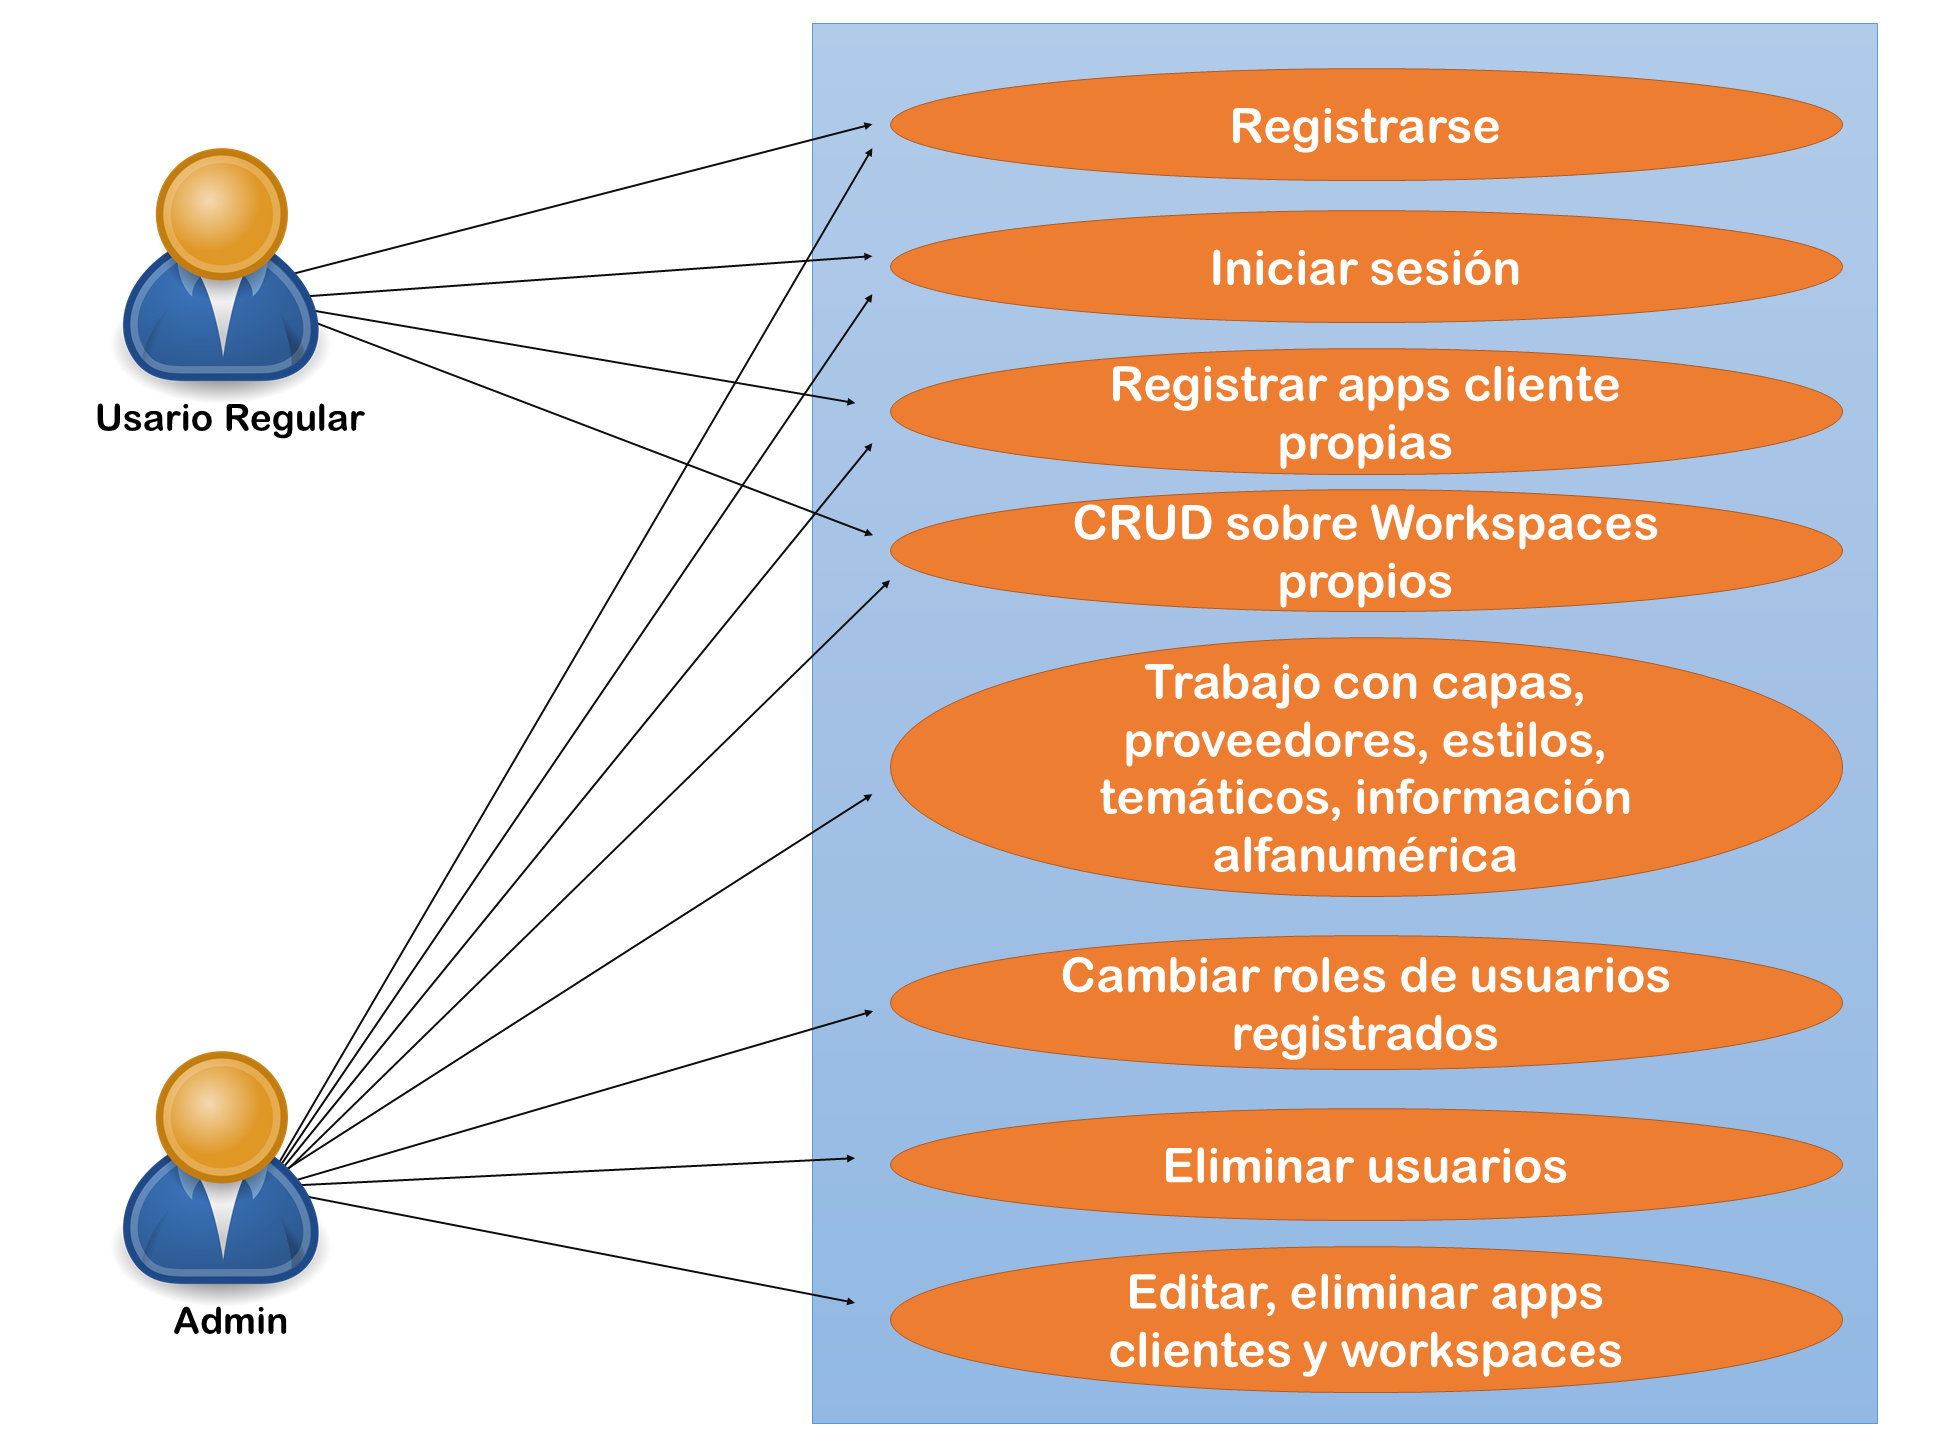
\includegraphics[width=0.52\textwidth]{images/casosdeUsousuario.png} 
\end{center} \vspace{-20pt} \caption{Diagrama de casos de uso de los usuarios en OLS.} \label{casos1}\vspace{-10pt} 
\end{wrapfigure}

Un administrador, adem\'as de realizar todas las acciones de un usuario regular, tambi\'en tiene acceso a las siguientes funcionalidades:

$\bullet$ Crear, editar, eliminar capas, proveedores de datos, estilos, tem\'aticos e informaci\'on alfanum\'erica.

$\bullet$ Cambiar roles de los usuarios registrados en el sistema o eliminarlos totalmente del servidor.

$\bullet$ Tiene acceso a todos los workspaces creados por los usuarios, as\'i como a todas las aplicaciones cliente registradas, pudiendo realizar cambios sobre estos.


\subsection{Aplicaciones cliente}
Los permisos que tienen las aplicaciones cliente para acceder a los servicios de OLS son controlados mediante workspaces. Un Workspace permite restringir las capas y funcionalidades del sistema. Todo cliente que se registra en el nuevo servidor de OpenLatino adquiere acceso a un Workspace llamado \textit{common}. Este espacio de trabajo cuenta con un m\'inimo de funcionalidades y capas para que el cliente pueda usar. Adem\'as, como ya se dijo, el usuario que registr\'o la aplicaci\'on puede crear nuevos Workspaces y as\'i darle acceso a m\'as capas y servicios.

\begin{wrapfigure}{l}{0.5\textwidth} 
\vspace{-20pt} 
\begin{center} 
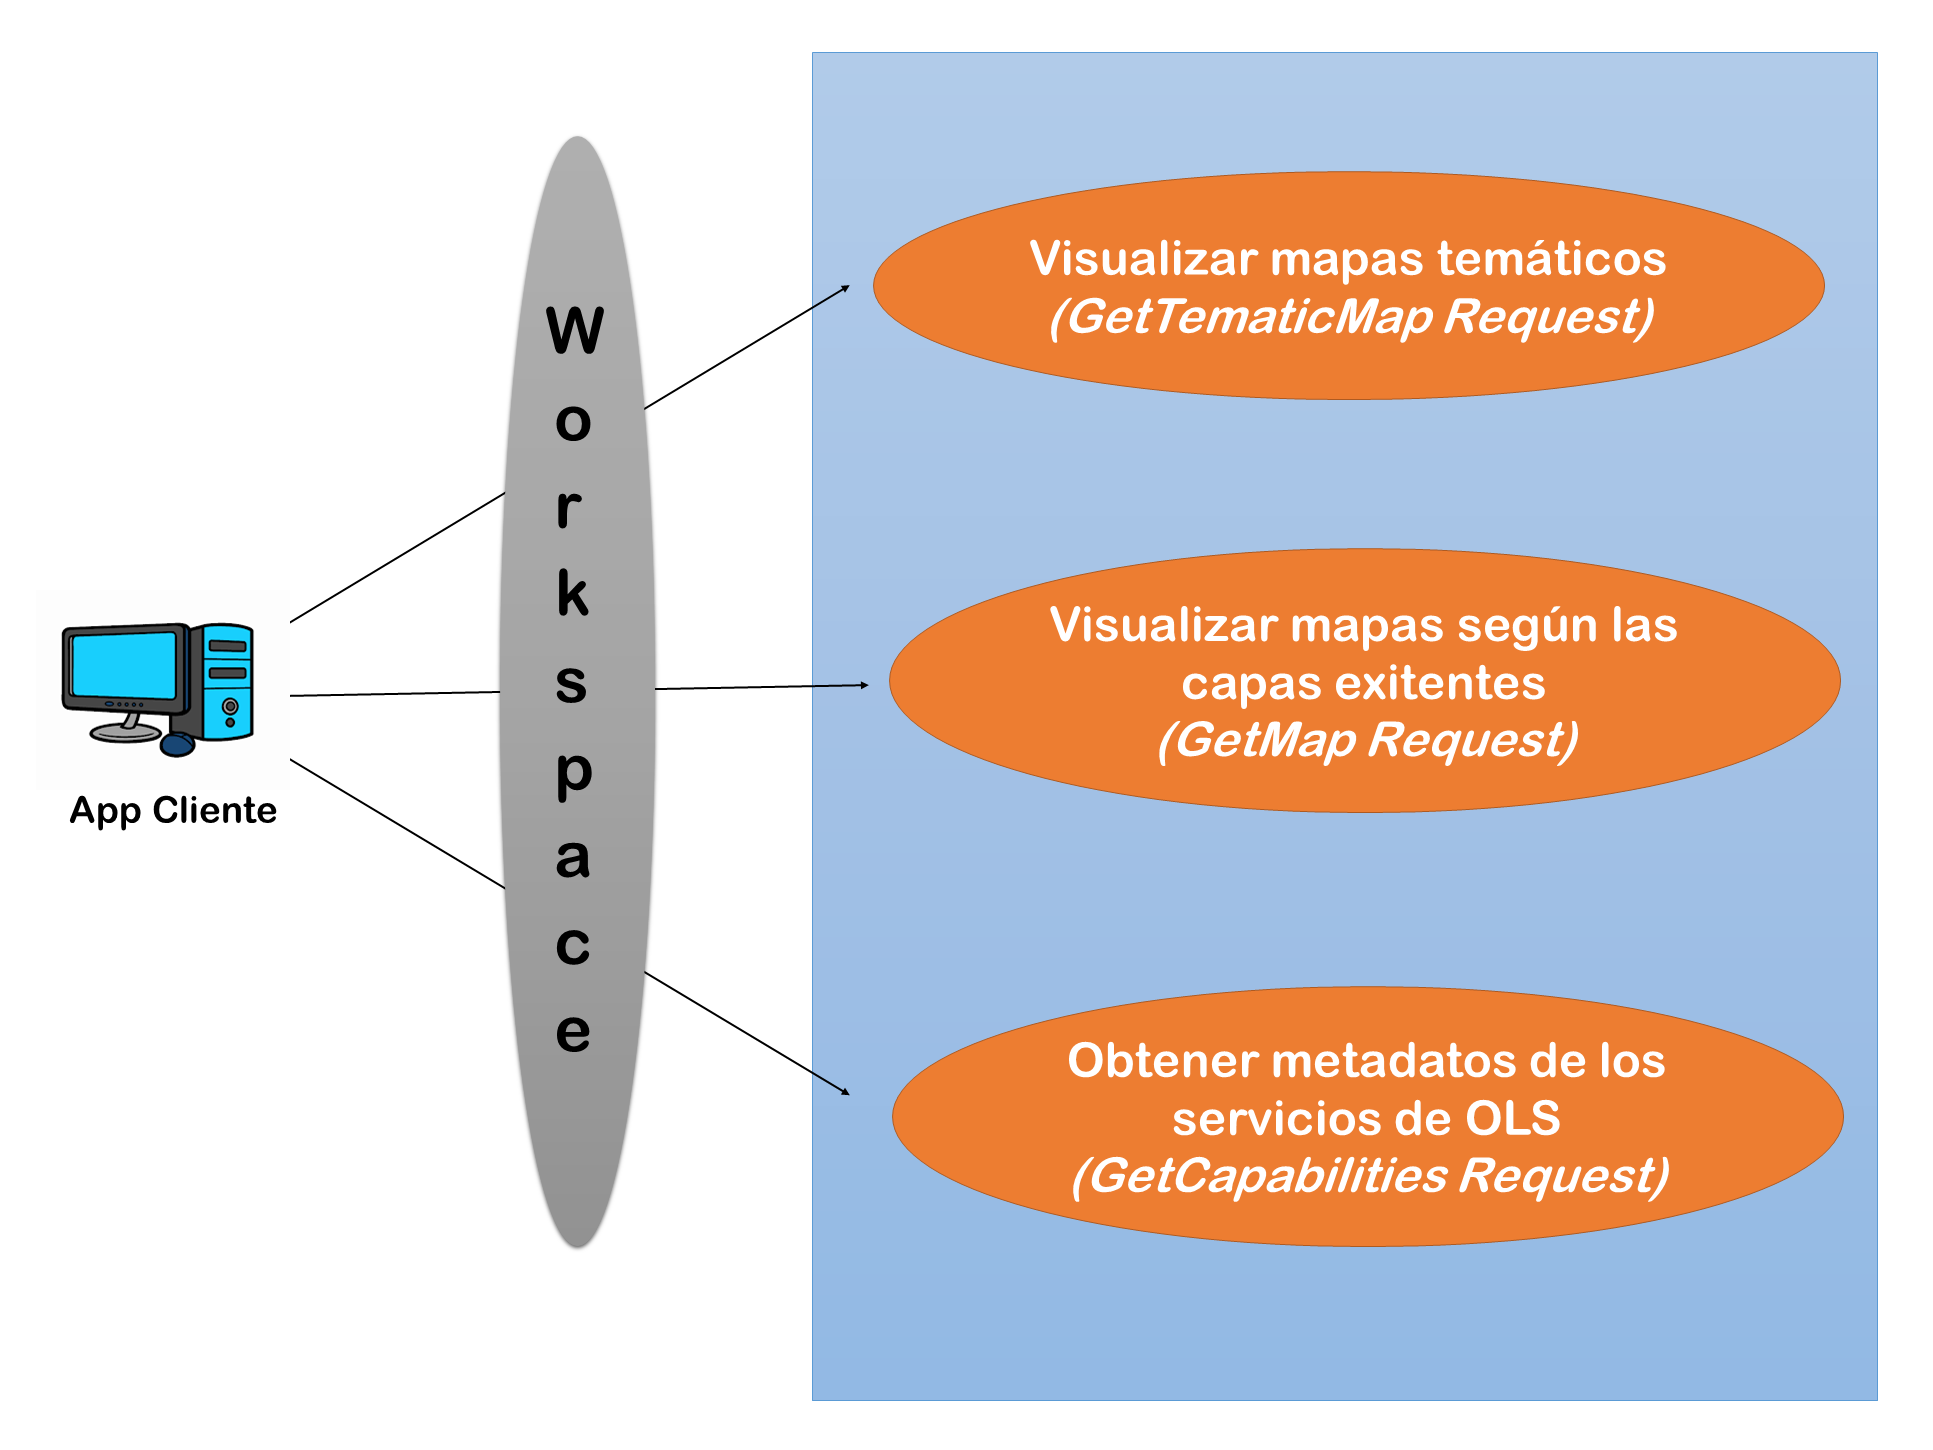
\includegraphics[width=0.52\textwidth]{images/casosdeUsoclient.png} 
\end{center} \vspace{-20pt} \caption{Diagrama de casos de uso de las aplicaciones cliente en OLS.} \label{casos2} \vspace{-10pt} 
\end{wrapfigure}

Cada aplicaci\'on cliente tiene uno o m\'as Workspaces asignados. Como se observa en la figura \ref{casos2}, una aplicaci\'on cliente, con todos los permisos posibles permitidos, tiene acceso a las siguientes funcionalidades:

$\bullet$ Visualizar mapas tem\'aticos definidos en el sistema. (Pedido GetTematicMap)

$\bullet$ Visualizar mapas seg\'un las capas registradas en el servidor. (Pedido GetMap)

$\bullet$ Obtener metadatos de los servicios que ofrece el servidor. (Pedido GetCapabilities)



\section{Modificaci\'on al modelo de datos}
Con el objetivo de crear una herramienta extensible para la creaci\'on de otros tipos de mapas tem\'aticos y, para evitar guardar informaci\'on repetida innecesariamente en la base de datos, se hace necesario la modificaci\'on del modelo de entidades relacionales (MER)\footnote{Herramienta para el modelo de datos, la cual facilita la representaci\'on de entidades de una base de datos.}

\begin{wrapfigure}{l}{0.5\textwidth} 
\vspace{-20pt} 
\begin{center} 
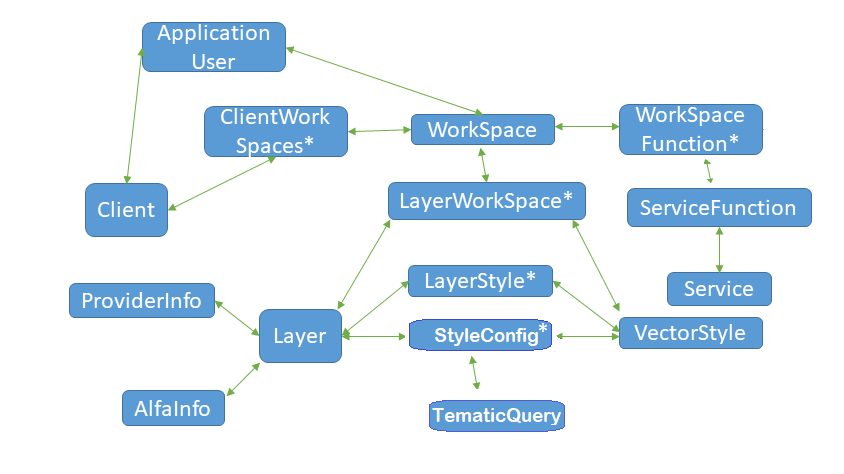
\includegraphics[width=0.53\textwidth]{images/merViejo.png} 
\end{center} \vspace{-20pt} \caption{Modelo de datos de la \'ultima versi\'on de OLS.} \label{merViejo} \vspace{-10pt} 
\end{wrapfigure}

Como se observa en la figura \ref{merViejo}, los tem\'aticos existentes se guardaban en la tabla \textit{TematicQuery}, la cual contiene el nombre del tem\'atico, y una funci\'on serializada que representa la consulta. De esta forma, en la tabla \textit{StyleConfig} se definen los estilos de cada tem\'atico mediante una llave for\'anea al \texttt{Id} de la tabla de tem\'aticos. 

En esta nueva versi\'on de OLS se redefinieron los mapas tem\'aticos para que estos pudieran soportar varias consultas, las cuales, a su vez, puedan soportar varios filtros separados por los operadores AND y OR. La figura \ref{merNuevo} muestra la base de datos modificada, mostrando en color rojo las tablas que sufrieron alguna variaci\'on y en color naranja las tablas que se crearon nuevas. 

\begin{wrapfigure}{l}{0.5\textwidth} 
\vspace{-20pt} 
\begin{center} 
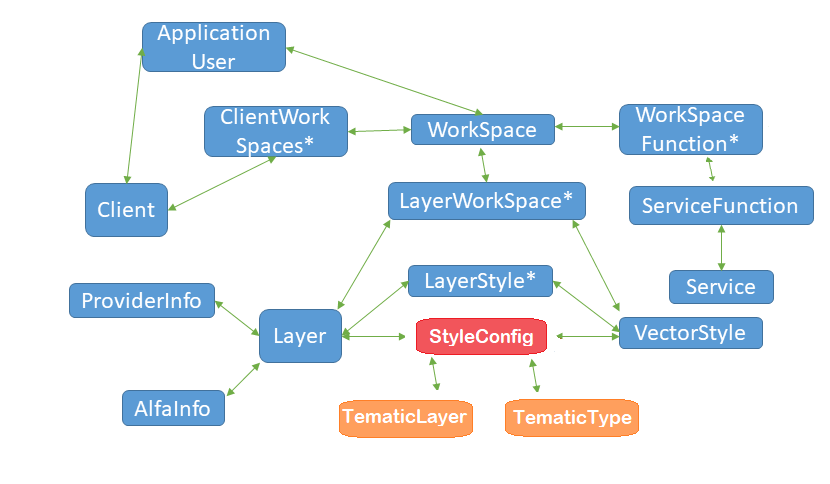
\includegraphics[width=0.53\textwidth]{images/merNuevo.png} 
\end{center} \vspace{-20pt} \caption{Modelo de datos modificado.} \label{merNuevo} \vspace{-10pt} 
\end{wrapfigure}

La tabla \textit{TematicQuery} se elimina, diviendo su contenido en dos nuevas tablas, contendiendo estas, adem\'as, informaci\'on acerca del tipo de tem\'atico.

Se a\~nadi\'o la tabla \textit{TematicLayers}, que representa el concepto de mapa tem\'atico, est\'a conformada por los campos \texttt{Name}, de tipo string y que representa su nombre, e \texttt{Id} que es su identificador de tipo num\'erico. Esta tabla tiene una relaci\'on de uno a muchos con \textit{StyleConfig}, ya que un tem\'atico tiene una o varias configuraciones de estilo, una para cada consulta. Tambi\'en, se cre\'o la tabla \textit{TematicTypes} la cual contiene la informaci\'on de los tem\'aticos, sus filtros, y el tipo de tem\'atico que representa. Esta relacionada con la tabla \textit{StyleConfig} en una relaci\'on de uno a muchos.

Como resultado de la incorporaci\'on de nuevas tablas relacionadas con \textit{StyleConfig}, esta tabla se modific\'o, conteniendo en esta nueva versi\'on la capa, el estilo, y el filtro asociado a un tem\'atico espec\'ifico, como llaves for\'aneas de las respectivas tablas.


\section{Arquitectura de software}
La arquitectura de software es el conjunto de estructuras necesarias para dar sentido a un sistema, lo cual abarca los elementos del software, las relaciones entre ellos y las propiedades de ambos. La arquitectura en capas es una de las m\'as utilizadas, esta se enfoca en la distribuci\'on de roles y responsabilidades de forma jer\'arquica dando una forma muy efectiva de separaci\'on de responsabilidades. El rol indica el modo y tipo de interacci\'on con otras capas, y la responsabilidad indica la funcionalidad que est\'a siendo desarrollada. \cite{architecture2}

\begin{wrapfigure}{l}{0.5\textwidth} 
\vspace{-20pt} 
\begin{center} 
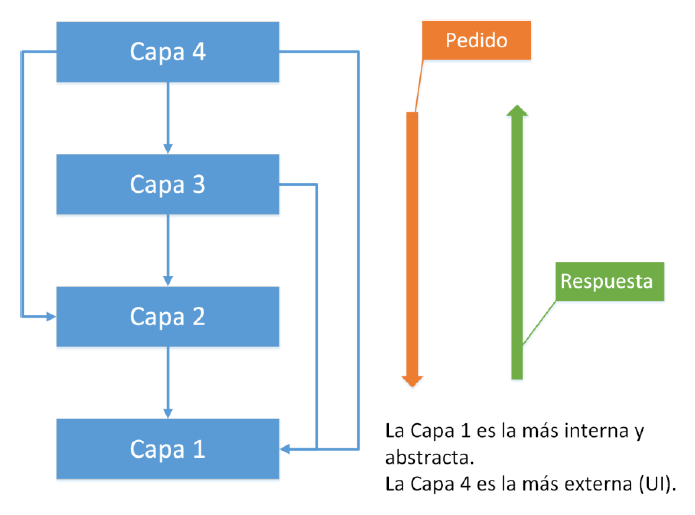
\includegraphics[width=0.52\textwidth]{images/arquitecturaFlexible.png} 
\end{center} \vspace{-20pt} \caption{Ejemplo de Arquitectura de capas con 4 capas en su forma flexible.} \label{flexible} \vspace{-10pt} 
\end{wrapfigure}

En una arquitectura de capas, todas las capas se colocan de forma horizontal, donde una capa solo puede depender otra que est\'e por debajo de ella, nunca por encima. En una forma estricta de la arquitectura, solo se puede acceder a la capa que est\'a exactamente debajo. Si se usa un acercamiento m\'as flexible, como se puede observar en la Figura \ref{flexible}, una capa puede acceder a todas las capas por debajo de ella. \cite{architecture}

La arquitectura de capas divide la aplicaci\'on con la intenci\'on de que cada una tenga un rol muy definido, no define la cantidad de capas que debe tener la aplicaci\'on y aplica el principio de separaci\'on de preocupaciones. La ventaja principal de este estilo es que el desarrollo se puede llevar a cabo en varios niveles y, en caso de tener que hacer alg\'un cambio, solo se realiza en el nivel que le corresponda.

\subsection{Modificaciones a la arquitectura de OLS}
OpenLatino Server implementa \textit{Clean Architecture}\footnote{Arquitectura limpia en espa\~nol. Presentada por Robert C. Martin (Uncle Bob) en su blog, el 13 de agosto de 2012 \cite{cleanArchitecture}}, la cual es una arquitectura por capas.  En la figura \ref{cleanArchitecture} se muestra la Arquitectura de software \textit{Clean Architecture} implementada en OLS. Se puede observar la separaci\'on de las capas y la dependencia que existe entre ellas.

\begin{wrapfigure}{l}{0.5\textwidth} 
\vspace{-20pt} 
\begin{center} 
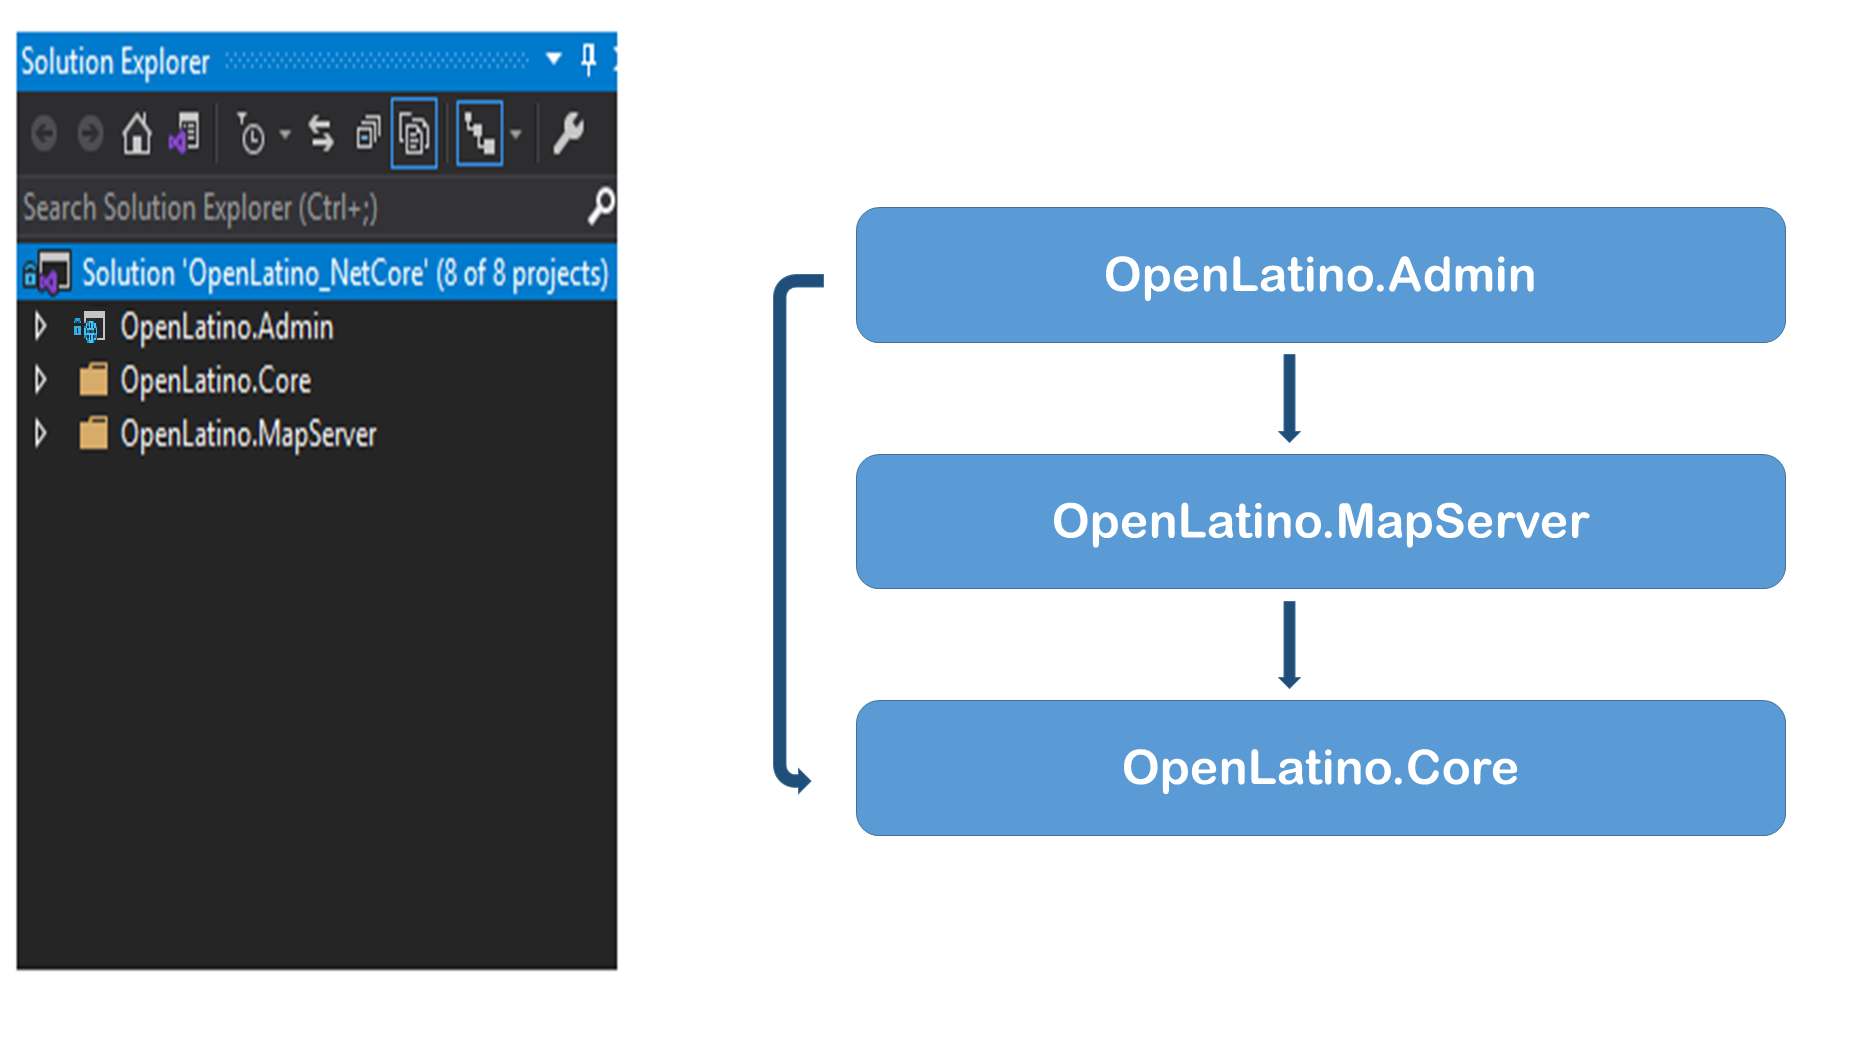
\includegraphics[width=0.53\textwidth]{images/cleanArchitecture.png} 
\end{center} \vspace{-20pt} \caption{Arquitectura de software \textit{Clean Architecture} implementada en OLS en su \'ultima versi\'on.} \label{cleanArchitecture} \vspace{-10pt} 
\end{wrapfigure}

En la \'ultima versi\'on, OLS presenta tres capas:

$\bullet$ \textbf{OpenLatino.Core}. Es la capa base. No tiene dependencias externas. Posee las entidades y la declaraci'on de las interfaces.

$\bullet$ \textbf{OpenLatino.MapServer.} Depende de la capa OpenLatino.Core. Se encarga de procesar los pedidos de las aplicaciones cliente y devolver un response. Posee la implementaci\'on de las funciones WMS.

$\bullet$ \textbf{OpenLatino.Admin}. Depende de las capas anteriores, posee la implementaci\'on de los controladores encargados de recibir las peticiones de las aplicaciones cliente.

En la nueva versi\'on de OLS, con la implementaci\'on de la interfaz visual de configuraci\'on en Angular, se hizo necesario modificar la arquitectura, manteniendo los principios de \textit{Clean Architecture}, garantizando la extensibilidad, seguridad y buenas pr\'acticas del servidor. La nueva arquitectura de OLS se muestra en la figura \ref{cleanArchitectureNew}.

Se elimin\'o la capa m\'as externa de la arquitectura de OLS y, en su lugar, se implementaron tres nuevas capas:

$\bullet$ \textbf{OpenLatino.Admin.Infraestructure}. Consiste en una capa de abstracci\'on entre la entre la capa de entidades de dominio y la capa de l\'ogica de negocio. Implementa el patr\'on Repositorio \footnote{Patr\'on de dise\~no que a\'isla la capa de datos del resto de la aplicaci\'on.}, que consulta la fuente de datos, los asigna a una entidad y realiza cambios en dicha entidad a la fuente de datos.

\begin{wrapfigure}{l}{0.5\textwidth}
\vspace{-20pt}
\begin{center}
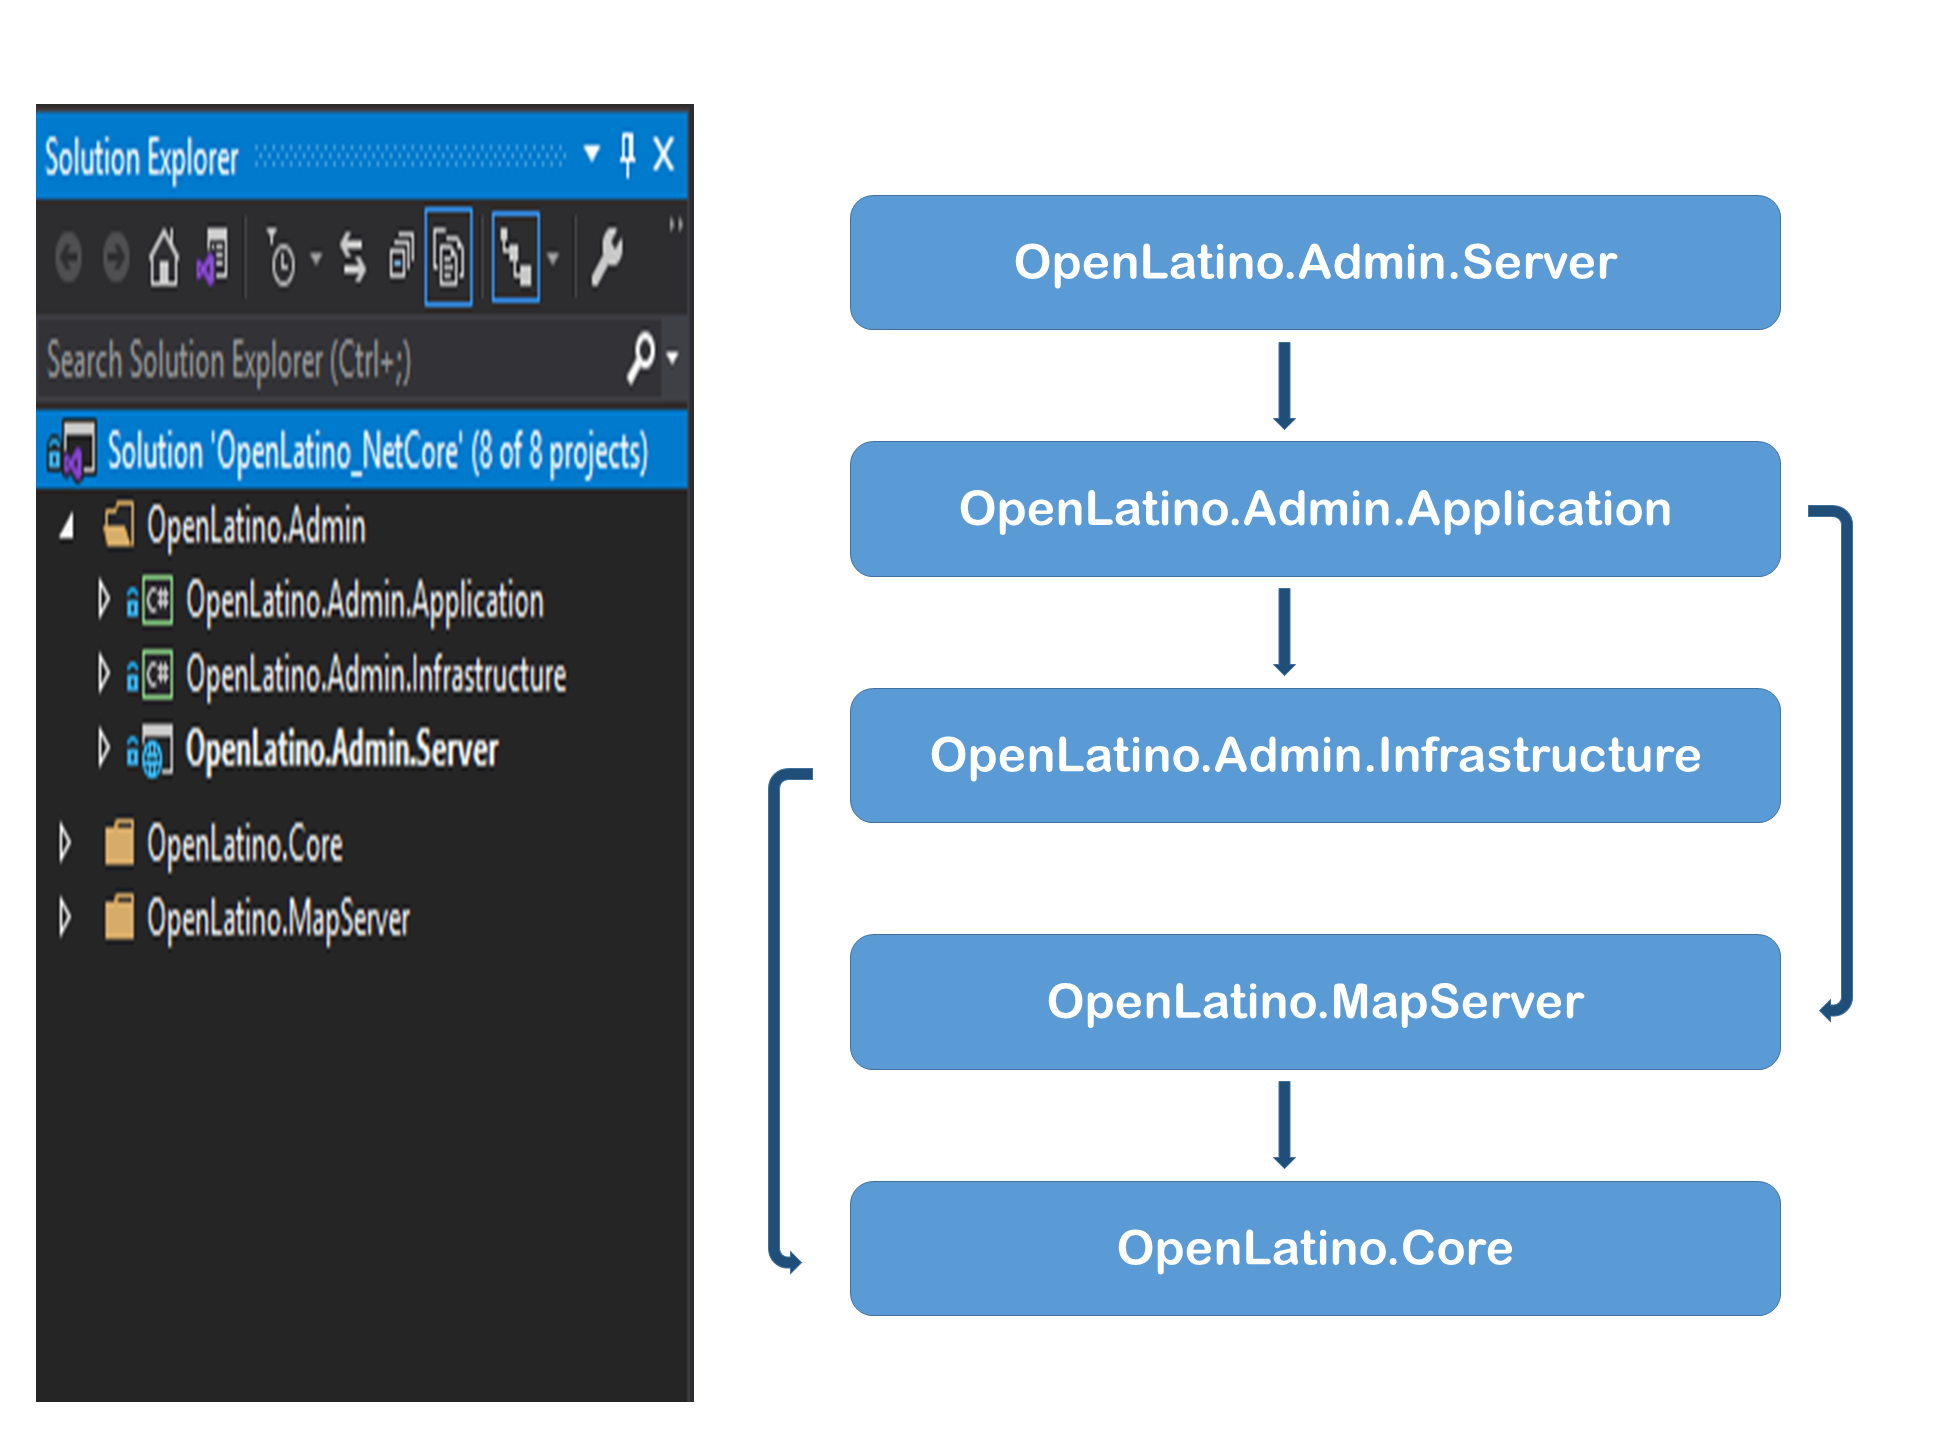
\includegraphics[width=0.52\textwidth]{images/cleanArchitectureNew.png} 
\end{center} \vspace{-20pt} \caption{Arquitectura de software \textit{Clean Architecture} de OLS modificada.}  \label{cleanArchitectureNew} \vspace{-10pt} 
\end{wrapfigure}

$\bullet$ \textbf{OpenLatino.Admin.Application}. Esta capa contiene interfaces que se utilizan para comunicarse entre la capa OpenLatino.Admin.Server y la capa de repositorio. Contiene los servicios asociados a una entidad espec\'ifica, ya sean proveedores, tem\'aticos, estilos, etc.

$\bullet$ \textbf{OpenLatino.Admin.Server} Es la capa m\'as externa de la aplicaci\'on, contiene los controladores que reciben los pedidos de las aplicaciones clientes y de los usuarios de la interfaz visual de configuraci\'on. En esta capa se realiza, adem\'as, la verificaci\'on de seguridad, que valida la identidad de los usuarios y clientes que realizan los pedidos.


\subsection{Arquitectura de la Interfaz Visual de Configuraci\'on.}
Las aplicaciones creadas con Angular se separan en plantillas HTML, clases de componentes en TypeScript, escritas para gestionar dichas plantillas, y los servicios que contienen la l\'ogica para la comunicaci\'on con el servidor. 

Para crear la interfaz visual se generaron templates con HTML, controlando estos con l\'ogica creada en componentes, que ser\'an exportados como clases. As\'i mismo, se agregan los servicios para manejar el flujo de datos de la aplicaci\'on y el servidor OLS. Finalmente, se ''encapsulan'' dichas componentes y servicios en m\'odulos. 

\begin{wrapfigure}{l}{0.5\textwidth}
\vspace{-20pt}
\begin{center}
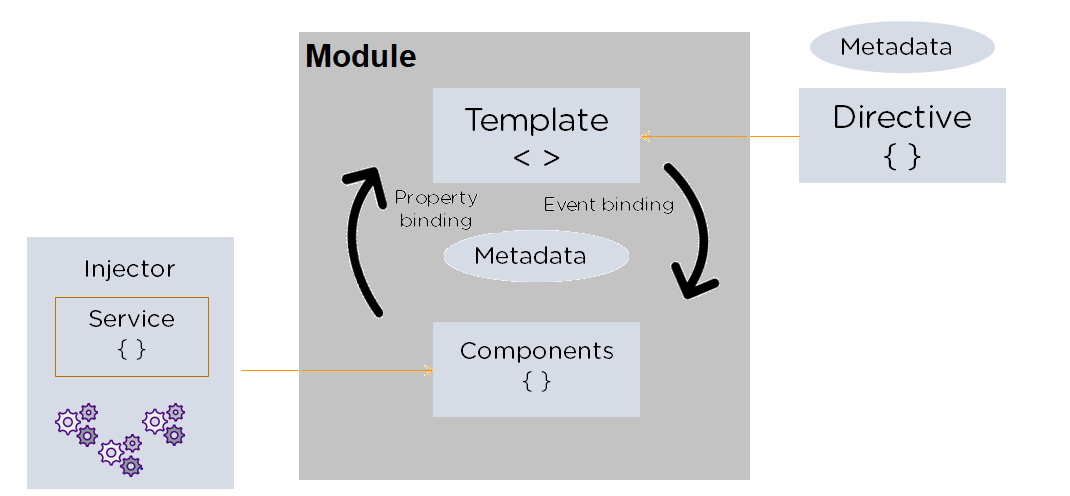
\includegraphics[width=0.52\textwidth]{images/angularArchitecture.png} 
\end{center} \vspace{-20pt} \caption{Arquitectura de software de la interfaz visual.}  \label{arquitecturaAngular} \vspace{-10pt} 
\end{wrapfigure}

La arquitectura de la aplicaci\'on desarrollada se muestra en la figura \ref{arquitecturaAngular}. Con el objetivo de seguir las buenas pr\'acticas de la programaci\'on, la interfaz visual implementa varios m\'odulos cuyas funcionalidades est\'an bien definidas e independientes. Estos gestionan el trabajo con tem\'aticos, estilos, proveedores, informaci\'on alfanum\'erica, auntenticaci\'on, etc\'etera. Cada uno de dichos m\'odulos contiene uno o varios servicios que se encargan de realizar los pedidos al servidor, atendiendo a las peticiones del usuario, y de recibir la respuesta de OLS. Estos servicios son inyectados en las componentes como dependencias.

Las componentes son clases que contienen la plantilla de la vista, y la l\'ogica asociada a esta, de una parte de la interfaz visual. Para gestionar la configuraci\'on de OLS se crearon varias componentes, encargadas de crear nuevos tem\'aticos, editar estilos, registrar usuarios, etc\'etera. En la interfaz visual, las plantillas HTML contienen directivas que le proveen l\'ogica de programaci\'on, las cuales realizan \textit{data binding}, es decir, enlazan la l\'ogica de los datos de la aplicaci\'on con las vistas. Por otro lado, \textit{event binding}, responde a la acci\'on del usuario al interactuar en la aplicaci\'on, actualizando los datos en la l\'ogica.


\section{Detalles de implementaci\'on}
En esta secci\'on se explicar\'an los cambios en el c\'odigo para la creaci\'on del nuevo tipo de mapa tem\'atico de categor\'ias, explicando el proceso para crear nuevos tipos de tem\'aticos. Se abordar\'a, tambi\'en, c\'omo fue implementada la seguridad de la interfaz visual y del servidor, no sin antes abordar en qu\'e consiste el est\'andar de seguridad JWT (JSON Web Token por sus siglas en ingl\'es).

\subsection{Implementaci\'on de mapas tem\'aticos}
Para crear el nuevo tipo de mapa tem\'atico se elimin\'o la entidad \texttt{TematicQuery}, creando en su lugar la nueva entidad \texttt{TematicType} (figura \ref{tematicType}), la cual contiene las propiedas inherentes a todo tipo de tem\'atico: Id, nombre, funci\'on, que constituye los filtros, y los estilos asociados. Se cre\'o, adem\'as, la entidad \texttt{TematicLayer} que contiene el nombre y el Id del tem\'atico.

\begin{wrapfigure}{l}{0.5\textwidth}
\vspace{-20pt}
\begin{center}
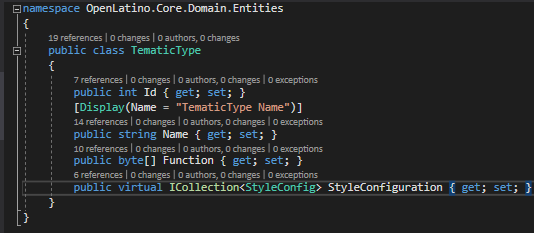
\includegraphics[width=0.52\textwidth]{images/tematicType.png} 
\end{center} \vspace{-20pt} \caption{Entidad que representa los tipos de tem\'aticos en OLS.}  \label{tematicType} \vspace{-10pt} 
\end{wrapfigure}

Para crear nuevos tem\'aticos se crea una nueva clase que herede de la nueva entidad \texttt{TematicType} (figura \ref{nuevosTipos}). 

\begin{wrapfigure}{l}{0.5\textwidth}
\vspace{-20pt}
\begin{center}
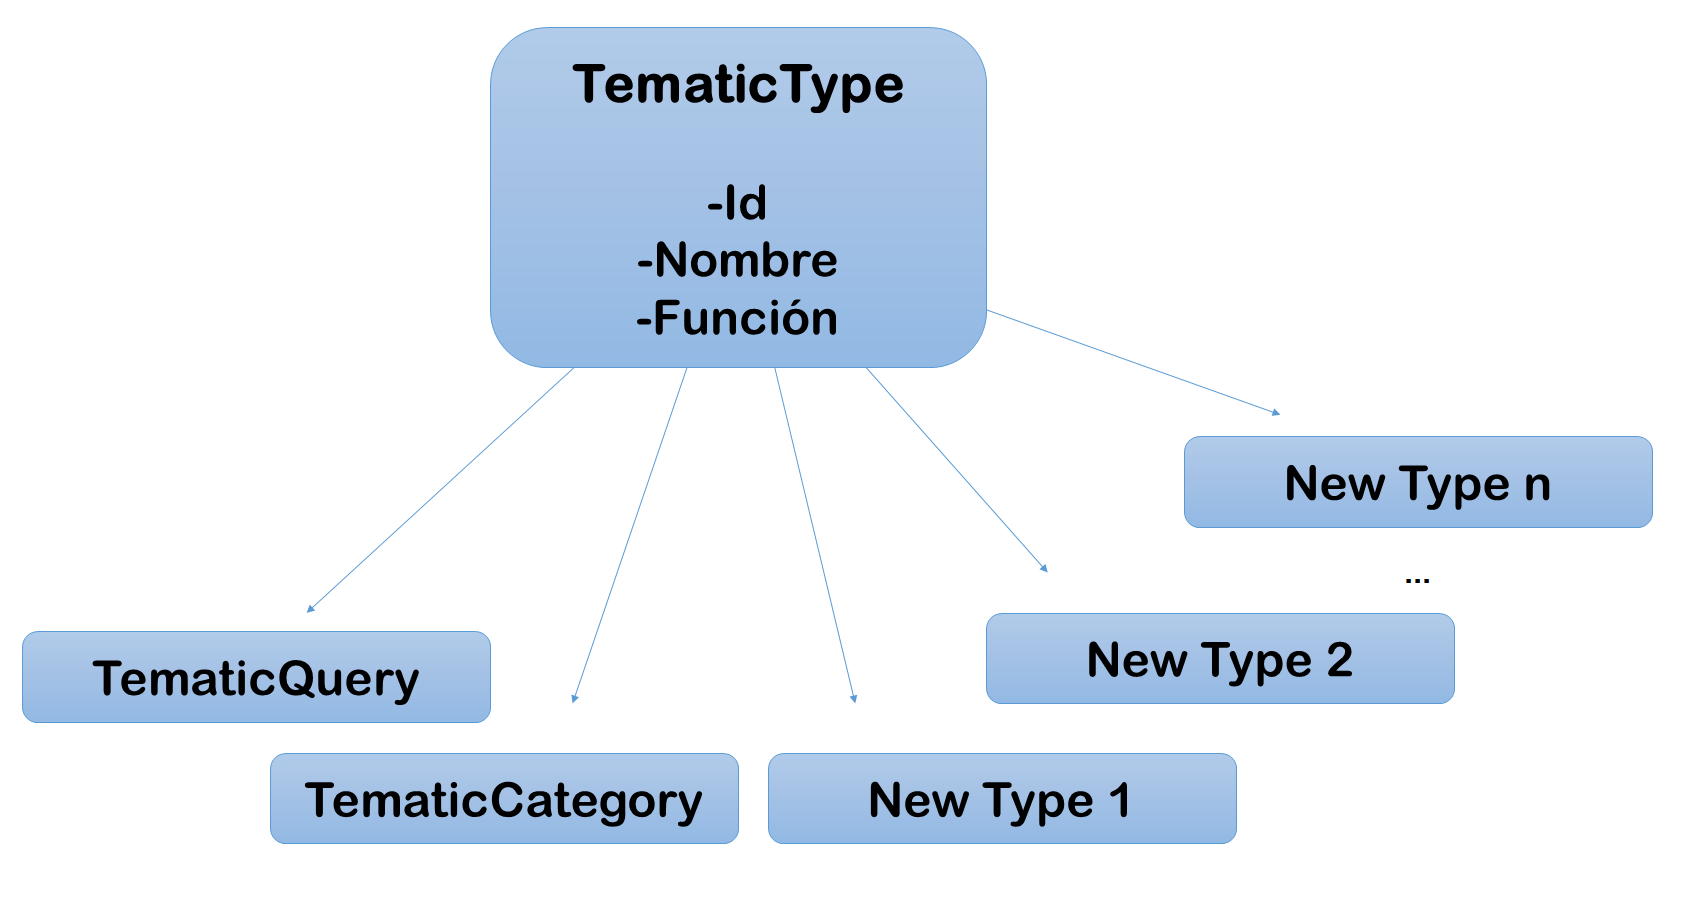
\includegraphics[width=0.52\textwidth]{images/newTematicTypes.png} 
\end{center} \vspace{-20pt} \caption{Estructura para crear nuevos tipos de mapas tem\'aticos.}  \label{nuevosTipos} \vspace{-10pt} 
\end{wrapfigure}

Al heredar de esta clase, autom\'aticamente la clase queda relacionada con la entidad \texttt{StyleConfig}, de esta manera no hay que modificar nada en la estructura existente: se crea la nueva entidad, se agrega alg\'un campo extra que necesite tener y se genera una nueva migraci\'on porque se modifica la base de datos existente al agregar el nuevo tipo.

Se crea, adem\'as, una interfaz \texttt{ITematicLayer Helper}, en sustituci\'on de la interfaz existente, que tiene los m\'etodos que permiten el trabajo con mapas tem\'aticos. El servicio \texttt{TematicLayerService} implementa esta interfaz. 

Para el procesamiento de nuevos tipos de tem\'aticos, se pueden seguir cualquiera de las siguientes v\'ias, dependiendo de lo que se desea implementar:

$\bullet$ \textbf{ITematicLayerHelper} $\rightarrow$ \textbf{TematicLayerService}. Usar el mismo servicio implementado para los tem\'aticos existentes.

$\bullet$ \textbf{ITematicLayerHelper} $\rightarrow$ \textbf{TematicLayerService} $\rightarrow$ \textbf{NewService}. Crear un nuevo servicio que use algunos m\'etodos del servicio existente, redefina otros y cree algunos nuevos.

$\bullet$ \textbf{ITematicLayerHelper} $\rightarrow$ \textbf{NewService}. Crear un nuevo servicio que tenga una implementaci\'on diferente de los m\'etodos actuales.

$\bullet$ \textbf{NewInterfaceHelper} $\rightarrow$ \textbf{NewService}. Crear una nueva interface, y un servicio que la implemente (para mantener la estructura de la aplicaci\'on) debido a que el nuevo tem\'atico usa m\'etodos diferentes a los definidos en la existente.

La opci\'on a escoger var\'ia de acuerdo a las necesidades del programador, dependiendo de las funcionalidades del nuevo tem\'atico a implementar.



\subsection{Seguridad de la interfaz visual y del servidor}
En esta nueva versi\'on de OLS es necesario implementar seguridad a nivel de Usuarios, para controlar las acciones que pueden realizar en la configuraci\'on del servidor desde la interfaz visual, y evitar pedidos de usuarios maliciosos. Igualmente se hace necesario implementar seguridad en los componentes de la interfaz visual, ya que un usuario no autorizado no puede acceder a algunas vistas restringidas en la aplicaci\'on. Para lograr lo anterior se decide implementar Json Web Token (JWT).

Json Web Token (JWT) es un est\'andar para transmitir informaci\'on de forma segura en internet, por medio de archivos en formato JSON\footnote{Tipo de archivo de texto plano con el cual se pueden crear par\'ametros y asignarles un valor}. Este sistema se utiliza en la autenticaci\'on de la interfaz visual, siendo su funci\'on principal la de validar la identidad de quien ingresa a la p\'agina, despu\'es de que ya haya iniciado sesi\'on en el pasado (figura \ref{login}). 

\begin{wrapfigure}{l}{0.5\textwidth}
\vspace{-20pt}
\begin{center}
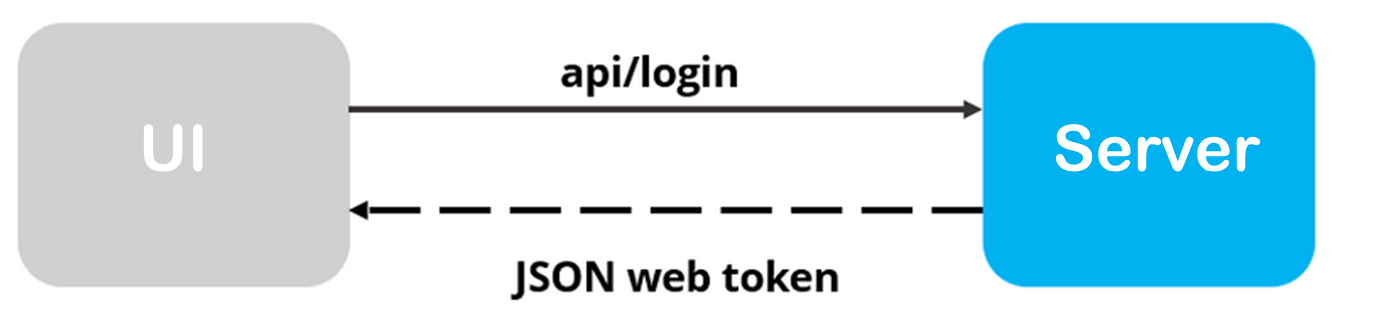
\includegraphics[width=0.52\textwidth]{images/login.png} 
\end{center} \vspace{-20pt} \caption{Login en OLS desde la interfaz visual.}  \label{login} \vspace{-10pt} 
\end{wrapfigure}

El contenido del token se encuentra firmado digitalmente, por lo que se puede comprobar su veracidad. Gracias a esta certificaci\'on, el servidor web puede aprobar de forma segura todas las peticiones que se hagan desde esa sesi\'on en nombre de ese usuario. Un JWT se divide en tres partes: el \textit{header}, que contiene el tipo de token y la informaci\'on del algoritmo de codificaci\'on\footnote{Usualmente HS256, que genera una firma sim\'etrica, esto quiere decir que el secret/key se usa tanto para el firmado como para la verificaci\'on de la firma.} usado. El \textit{Payload}, que contiene la informaci\'on relativa al usuario, si es admin o usuario regular, cuando inici\'o sesi'on, su Id en el sistema, etc\'etera.

\begin{wrapfigure}{l}{0.5\textwidth}
\vspace{-20pt}
\begin{center}
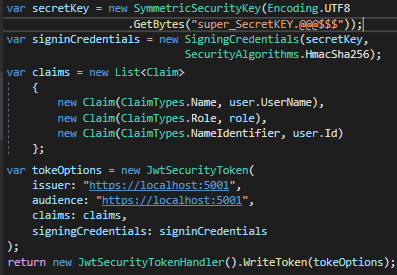
\includegraphics[width=0.52\textwidth]{images/jwtOLS.png} 
\end{center} \vspace{-20pt} \caption{JWT en OLS.}  \label{jwtOLS} \vspace{-10pt} 
\end{wrapfigure}

Finalmente, \textit{Signature} contiene la firma digital del token, creada combinando el header y el payload, basado en una clave secreta que solo el servidor conoce. Los JWT se generan en OLS cuando un usuario inicia sesi\'on en el sistema, la figura \ref{jwtOLS} muestra el fragmento de c\'odigo donde se crea el token y se retorna a la vista. \texttt{JwtSecurityToken} contiene importantes par\'ametros: los dos primeros son para verificar que OLS es el que esta respondiendo los pedidos a la vista, la tercera propiedad contiene informaci\'on acerca del usuario que inici\'o sesi\'on en el sistema; el \'ultimo par\'ametro contiene la firma digital.

A\'un con todas las comprobaciones que se realizan, existe un problema grave de seguridad, ya que un agente externo puede interceptar los pedidos que viajan a OLS desde la interfaz visual y obtener un token que no es suyo, esto implica que puede usarlo para realizar pedidos al servidor como si fuera ese cliente y acceder a informaci\'on confidencial sin ser detectado. 

Para resolver este problema se le establece un tiempo de vida limitado para cada token, es decir, cada uno de los tokens que se les entrega a los clientes ser\'a v\'alido solo por un tiempo prefijado. Este cambio garantiza que, si un token es robado, una vez que se agote su tiempo de vida, no servir\'a. En el caso de OLS, se a\~nade la propiedad \texttt{ expires: DateTime.Now.AddMinutes(30)} al JWT, lo que quiere decir que un usuario se mantendr\'a registrado en el sistema solo por media hora, pasado ese tiempo debe volver a ingresar mediante su contrase\~na.

\begin{wrapfigure}{l}{0.5\textwidth}
\vspace{-20pt}
\begin{center}
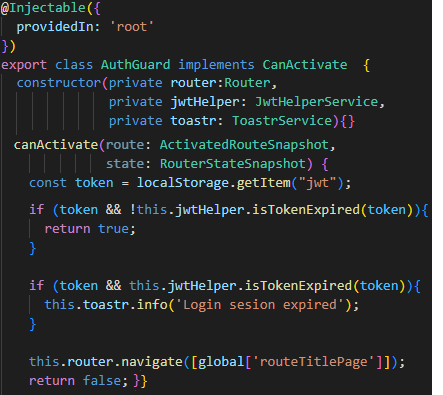
\includegraphics[width=0.52\textwidth]{images/authAngular.png} 
\end{center} \vspace{-20pt} \caption{Seguridad en la interfaz visual.}  \label{auth} \vspace{-10pt} 
\end{wrapfigure}

Del lado del FrontEnd tambi\'en se hacen verificaciones de seguridad, mediante el JWT enviado desde el servidor. Se realizan validaciones, permintiendo a los usuarios acceder a las  vistas de configuraci\'on, seg\'un sus roles. Un usuario que no est\'a logeado no puede acceder a ninguna vista de configuraci\'on, adem\'as, si no es administrador no puede acceder a todas las vistas. En el \texttt{app-routing-module}, mediante la propiedad \texttt{canActivate}, se reciben, por inyecci\'on de dependencia, las clases que verifican, de acuerdo al JWT, si el usuario tiene acceso a la ruta solicitada. En la figura \ref{auth} se muestra la clase encargada de verificar si un usuario esta logeado y si su sesi\'on no ha expirado.

Finalmente, se incluyen los los JWT en los pedidos del FrontEnd a OLS en el header de Autorizaci\'on\footnote{Authorization header, en ingl\'es, contiene las credenciales para autenticar a un usuario en un servidor}.

\begin{wrapfigure}{l}{0.5\textwidth}
\vspace{-20pt}
\begin{center}
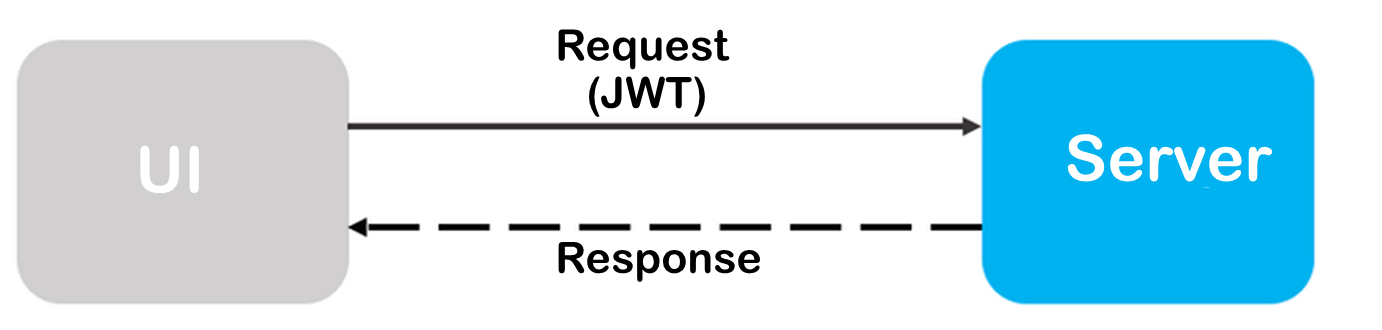
\includegraphics[width=0.52\textwidth]{images/request.png} 
\end{center} \vspace{-20pt} \caption{Pedido de la interfaz visual a OLS.}  \label{request} \vspace{-10pt} 
\end{wrapfigure}

Esto se hace con el objetivo de que el servidor valide que el pedido que se est\'a realizando proviene de la interfaz visual de configuraci\'on y no de un agente externo. (figura \ref{request})





 
%% Los cap'itulos inician con \chapter{T'itulo}, estos aparecen numerados y
%% se incluyen en el 'indice general.
%%
%% Recuerda que aqu'i ya puedes escribir acentos como: 'a, 'e, 'i, etc.
%% La letra n con tilde es: 'n.
\chapter{Pruebas de Funcionalidad}
En este cap\'itulo se realizan un conjunto de pruebas de correctitud y optimizaci\'on para demostrar el buen funcionamiento de las herramientas implementadas y as\'i evidenciar el cumplimiento de los objetivos planteados en el trabajo.

Las pruebas se realizaron en una laptop con las siguientes caracter\'isticas:
\begin{itemize}
\item Sistema operativo Windows 10 Enterprise LTSC, 64 bits.
\item Procesador Intel(R) Core(TM) i3-6100U @ 2.30GHz 2.30GHz.
\item Memoria RAM: 8GB (7.82 usable)
\item Disco duro 250GB, HDD.
\end{itemize}

Se cuenta con la cartograf\'ia de GeoCuba para las pruebas, las cuales iniciaron con los siguentes datos guardados en la base de datos de Admin: 
\begin{itemize}
\item Capa \textbf{Roads}(Calles), color rojo definido por defecto, con informaci\'on alfanum\'erica asociada de cinco columnas: \textit{maxspeed}, \textit{oneway}, \textit{bridge}, \textit{type}, \textit{name}.
\item Un usuario con rol de Administrador, \textit{adminopenlatino@gmail.com}.
\item Workspace \textit{AdminWorkspace}, asociado al usuario anterior, con acceso a las funciones \textit{GetCapabilities}, \textit{GetMap} y \textit{GetTematicMap}.
\item Estilos \textit{RedStyle}, \textit{BlueStyle}, \textit{GreenStyle} y \textit{YellowStyle} que representan los colores, rojo, azul, verde y amarillo respectivamente.
\end{itemize}

Para la validaci\'on de las pruebas se usar\'a Postman, verificando mediante este que el sistema est\'a funcionando correctamente. Postman es una aplicaci\'on que permite realizar pruebas API. Es un cliente HTTP\footnote{HTTP, de sus siglas en ingl\'es: Hypertext Transfer Protocol, es el nombre de un protocolo que permite realizar una petici\'on de datos y recursos.} que da la posibilidad de realizar \textit{HTTP requests} a trav\'es de una interfaz gr\'afica de usuario, por medio de la cual se obtiene la respuesta del servidor.

\section{Configuraci\'on de tem\'aticos por categor\'ias}
El objetivo de esta prueba es crear un nuevo tem\'atico en OLS. Se trabajar\'a sobre la capa \textbf{Roads}, escogiendo la columna \textit{oneway}\footnote{Seg\'un la cartograf\'ia de GeoCuba, este campo tiene valor 1 si la calle es de un solo sentido y 0 en caso contrario} como campo alfanum\'erico. La figura \ref{create} muestra la vista de creaci\'on con los datos anteriores.

\begin{figure}[h]
\centering
\label{create}
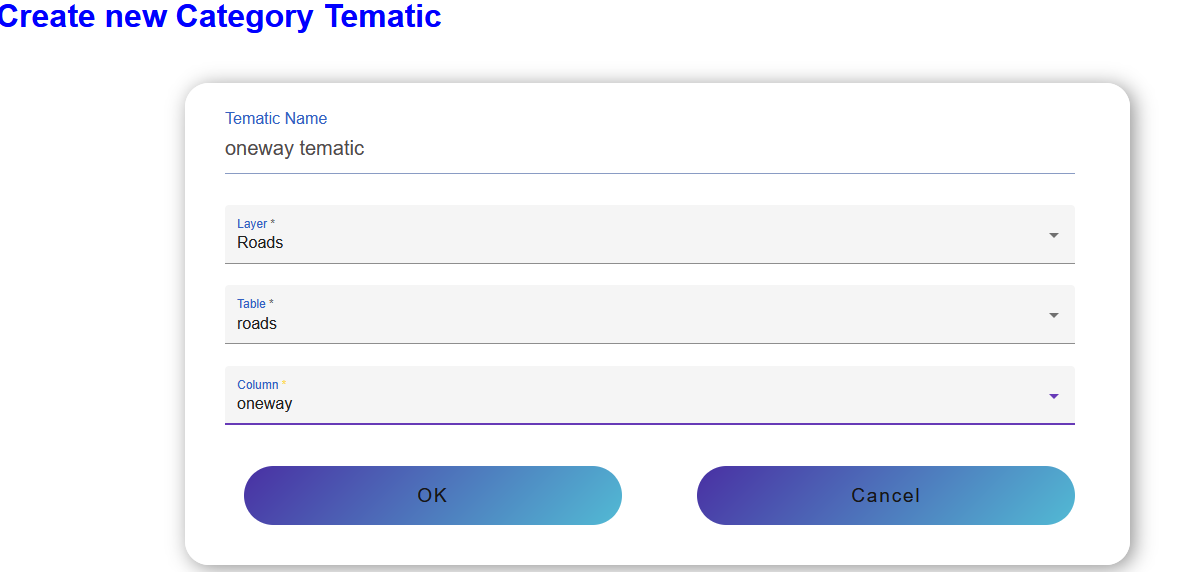
\includegraphics[scale=0.5]{images/createTematic.png} 
\caption{Vista de creaci\'on de tem\'aticos de categor\'ias.}
\end{figure}

Se espera que se genere una configuraci\'on de tem\'atico donde se tienen dos estilos para dos categor\'ias. Efectivamente, se comprueba que dando click en el bot\'on \textbf{OK}, se genera la configuraci\'on del tem\'atico autom\'aticamente, observ\'andose en la figura \ref{config} las dos posibles categor\'ias de la columna seleccionada, y la asignaci\'on de estilos. Si no hay suficientes estilos para cada categor\'ia el usuario puede generarlos desde esta vista. El usuario tambi\'en tiene la posibilidad de cambiar los estilos asignados por otros o crear uno nuevo.

\begin{figure}[h]
\centering
\label{config}
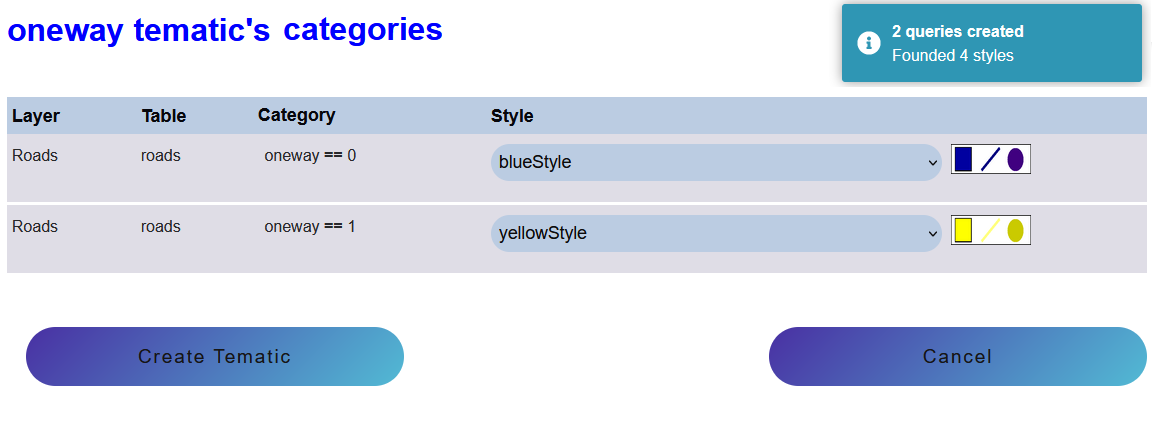
\includegraphics[scale=0.4]{images/configTematic.png}
\caption{Configuraci\'on generada a partir de los datos de la vista de creaci\'on.}
\end{figure}

Si se da click sobre el bot\'on \textbf{Create Tematic}, se genera el nuevo tem\'atico como se observa en la figura \ref{listTematic}. La cual muestra una lista de todos los tem\'aticos de ese tipo creados, en este caso, solo existe el tem\'atico de nombre \textit{oneway tematic}. Adem\'as, se observa la informaci\'on asociada a este: capa, categor\'ias, estilos, etc.

\begin{figure}[h]
\centering
\label{listTematic}
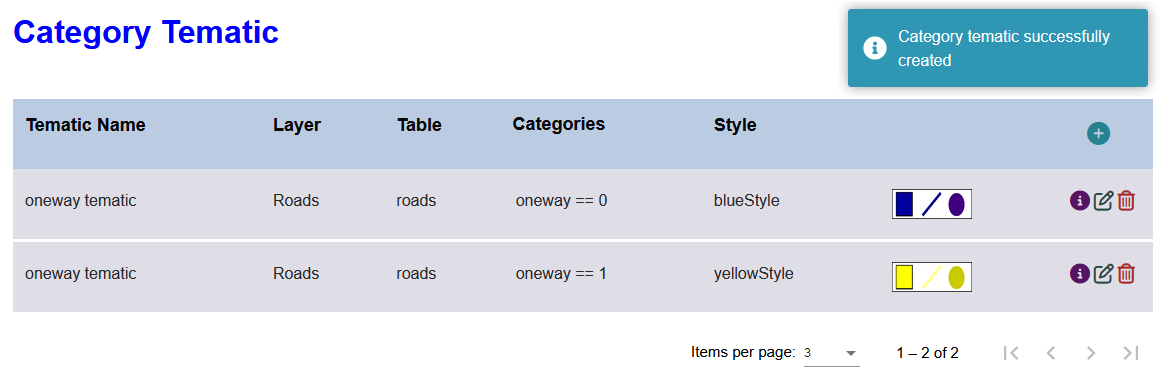
\includegraphics[scale=0.4]{images/listTematic.png} 
\caption{Listado de mapas tem\'aticos creados en OLS.}
\end{figure}


\section{Generaci\'on de mapas tem\'aticos por categor\'ias.}
Mediante postman se verifica que el tem\'atico creado en la secci\'on anterior se pinta bien sobre el mapa. Se espera que al realizar el pedido, se coloreen las calles de un solo sentido de azul y las de dos sentidos de amarillo. Si existe alguna calle que no tenga definido sentido en la cartograf\'ia, debido a que este valor es NULL, se pinta del valor por defecto de las calles, en este caso, rojo.

\begin{figure}[h]
\centering
\label{postmanTematic}
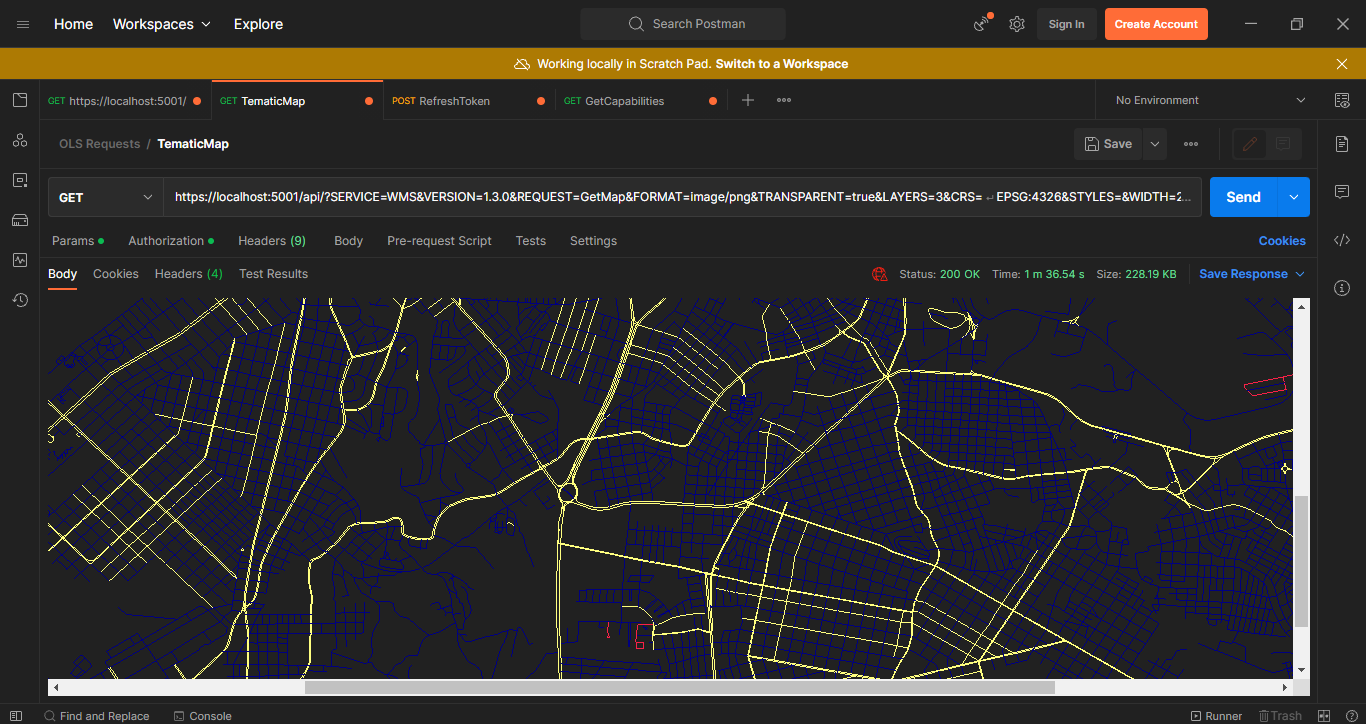
\includegraphics[scale=0.4]{images/postmanTematic.png} 
\caption{Pedido \textit{GetTematicMap.}}
\end{figure}

La figura \ref{postmanTematic} muestra la respuesta del servidor para el tem\'atico reci\'en creado. Se observan los resultados esperados. Ahora se edita el tem\'atico, para en lugar de pintar las calles de amarillo, lo haga de verde (figura \ref{editTematic}).

\begin{figure}[h]
\centering
\label{editTematic}
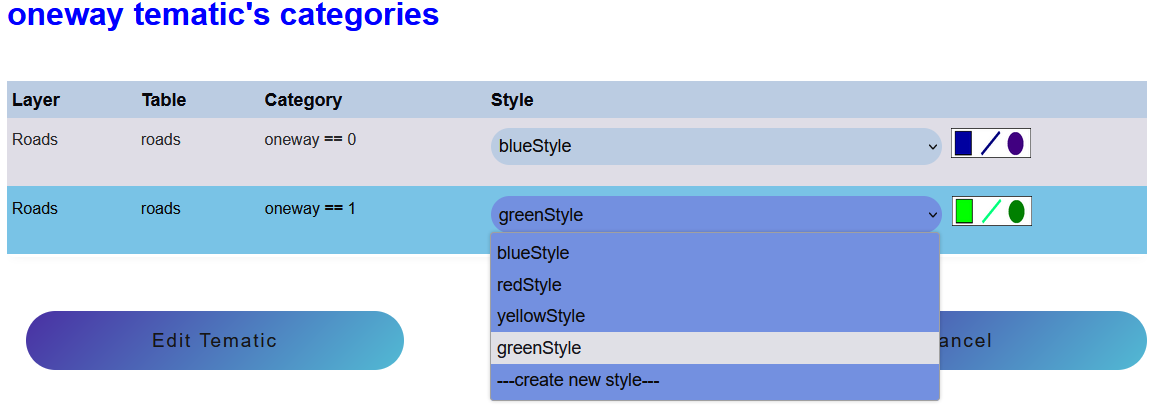
\includegraphics[scale=0.4]{images/editTematic.png} 
\caption{Edici\'on de tem\'aticos.}
\end{figure}

Si se realiza nuevamente el pedido se observa que ahora las calles de doble sentido est\'an coloreadas de verde.(figura \ref{postman2})

\begin{figure}[h]
\centering
\label{postman2}
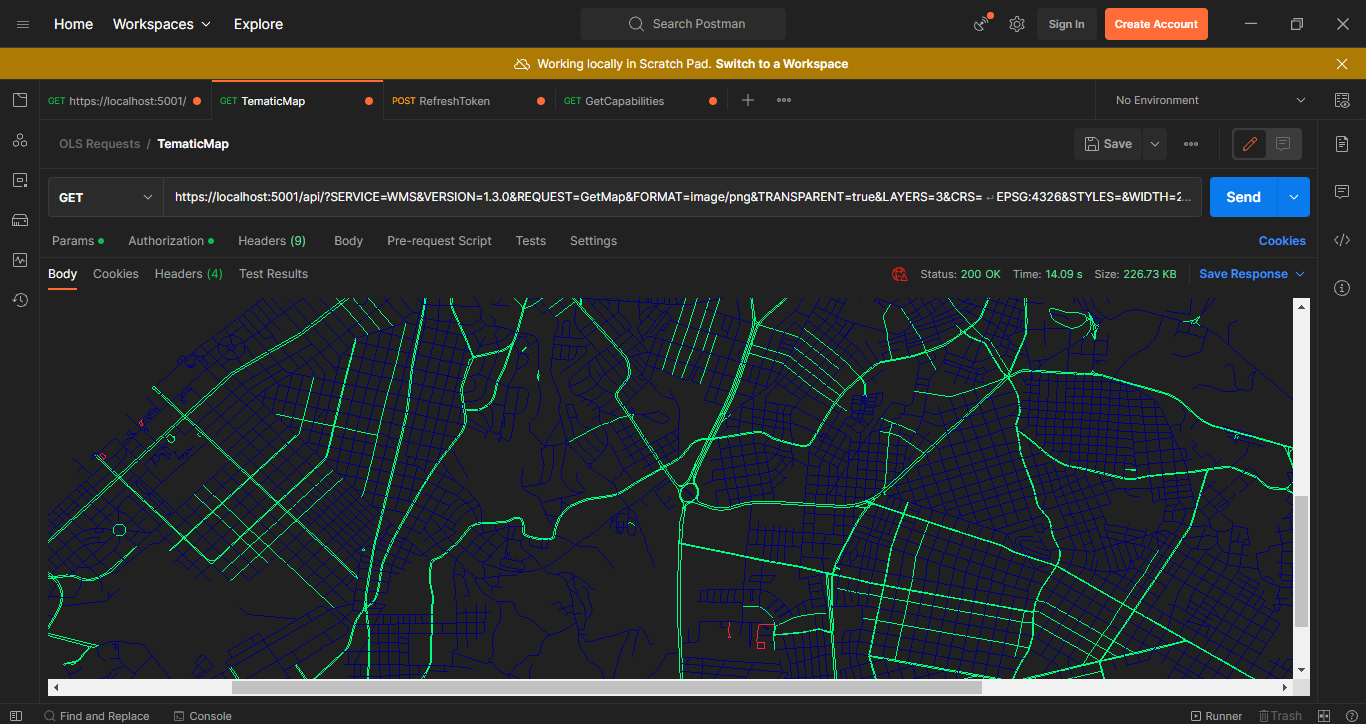
\includegraphics[scale=0.4]{images/postmanTematic2.png} 
\caption{Pedido \textit{GetTematicMap} a tem\'atico editado.}
\vspace{5cm}
\end{figure}



\section{Comprobaciones a la interfaz visual}
En esta prueba se verifica que la interfaz visual est\'a funcinando correctamente mediante operaciones CRUD. Para ello se trabaja con la entidad \textit{estilos}, y funciona de manera an\'aloga para el resto de las entidades. Primeramente, el estilo de color verde, se editar\'a y pasar\'a a ser de color celeste, elimin\'andolo finalmente del servidor.

La figura \ref{estilo} muestra la vista de edici\'on, y los listados de estilo despu\'es de editado. Se observan los resultados esperados. Finalmente, se eliminar\'a este estilo del sistema. La figura \ref{deleteStyle} muestra que esta operaci\'on se realiz\'o satisfactoriamente.

\begin{figure}[h]
\centering
\label{estilo}
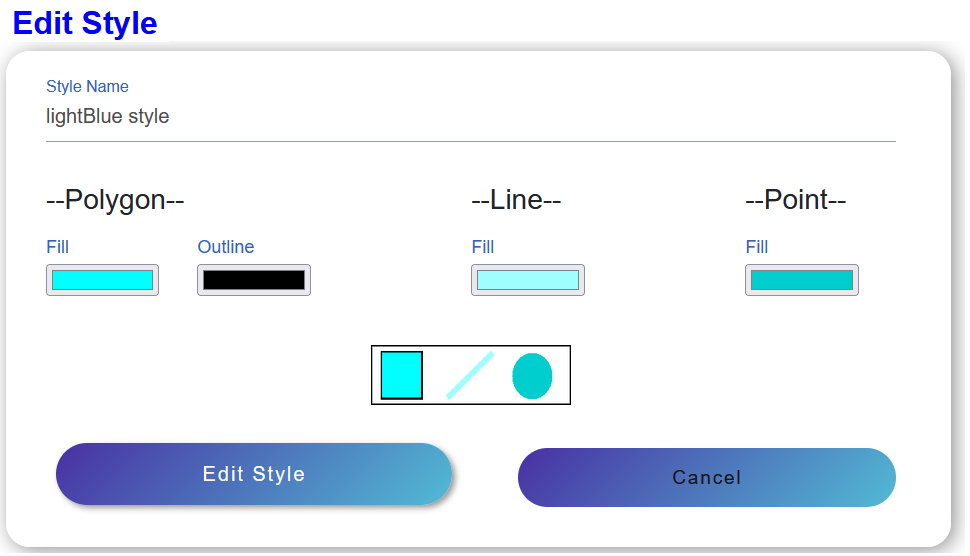
\includegraphics[scale=0.3]{images/editStyle.png} 
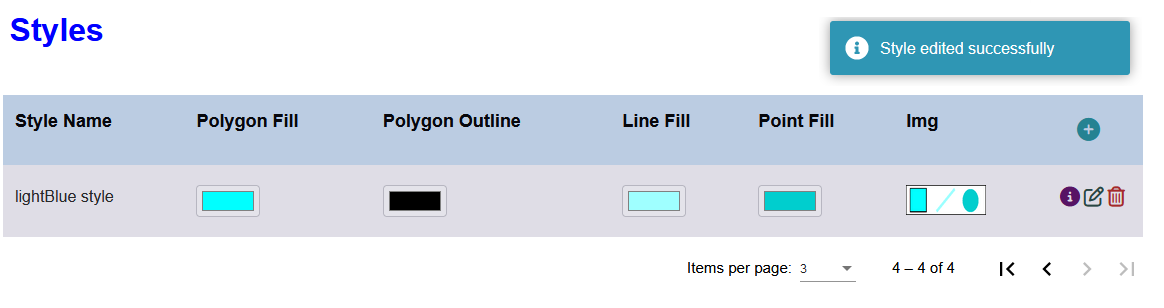
\includegraphics[scale=0.3]{images/listStyle.png} 
\caption{Edici\'on de estilos.}
\end{figure}

\begin{figure}[h]
\centering
\label{deleteStyle} 
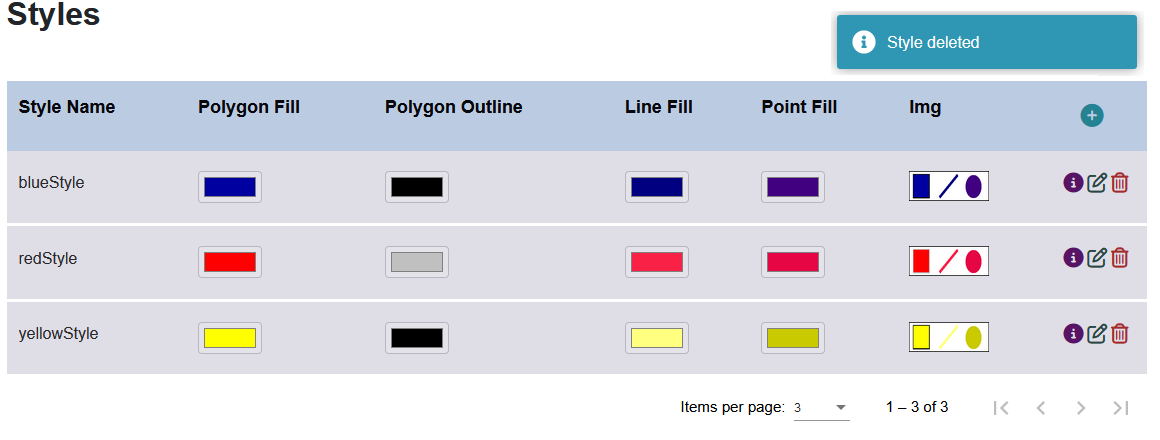
\includegraphics[scale=0.3]{images/deleteStyle.png} 
\caption{Eliminaci\'on de estilos.}
\end{figure}






%-------------------------------------------------------------------------------------------------------------------------------------
%-------------------------------------------------------------------------------------------------------------------------------------

\chapter{Conclusiones, recomendaciones y trabajo futuro}
La implementaci\'on de las funcionalidades expuestas en cap\'itulos anteriores da soluci\'on a las deficiencias planteadas de OLS, por lo tanto, se cumplieron los objetivos propuestos. 

En este cap\'itulo se exponen las conclusiones a las que se arribaron con el desarrollo de la aplicaci\'on y se proponen, adem\'as, algunas recomendaciones para el trabajo futuro con OLS.

\section{Conclusiones}
El presente trabajo de diploma finaliza con la creaci\'on de la nueva interfaz visual de OLS, intuitiva, agradable y segura. Para lograrlo, se realizaron modificaciones sobre el sistema, en su arquitectura, modelo de datos y desarrollo de nuevas funcionalidades, con una implementaci\'on extensible y reusable, manteniendo las buenas pr\'acticas que presenta el servidor. Se cre\'o, adem\'as, un nuevo tipo de tem\'atico, por clasificaci\'on de tipos o por categor\'ias, que le permite al usuario la creaci\'on de mapas tem\'aticos de forma sencilla, ya que todo el procesamiento de los datos y asignaci\'on de estilos se realiza de forma autom\'atica,  extendiendo, para lograr este prop\'osito, el \textit{Render}(clase encargada de pintar los mapas) de OLS, para que aceptara filtros gen\'ericos, en lugar de consultas sql. Por \'ultimo, se modific\'o el pedido \textit{GetCapabilities} para que este muestre tambi\'en la informaci\'on acerca de los tem\'aticos existentes, tambi\'en se cre\'o un nuevo pedido \textit{GetTematicCapabilities}, que devuelve solo la informaci\'on de los mapas tem\'aticos creados.

Estos cambios mencionados dotan a OLS de mejoras y nuevas funcionalidades, por lo que se puede concluir que los principales aportes de esta investigaci\'on son:

\begin{itemize}
\item Modificaci\'on del pedido \textit{GetCapabilities} para que devuelva informaci\'on acerca de mapas tem\'aticos y creaci\'on de un nuevo pedido que devuelve solo esa informaci\'on.
\item Implementaci\'on de una nueva interfaz visual, mediante la cual se puede modificar la configuraci\'on de OLS de forma intuitiva.
\item Creaci\'on de un nuevo tipo de mapa tem\'atico que realiza el procesamiento de capas, categor\'ias asociadas y estilos autom\'aticamente.
\item Modificaci\'on de la arquitectura de OLS para acoplar la nueva interfaz visual, implementada en Angular, y la seguridad de los pedidos de los usuarios.
\item Cambio del modelo de datos para la implementaci\'on del nuevo tem\'atico y hacer extensible el proceso de agregar nuevos tipos.
\item Nueva implementaci\'on del Render para que acepte filtros gen\'ericos (varias condiciones separadas por operadores l\'ogicos) en lugar de consultas sql.
\end{itemize}


\section{Recomendaciones y trabajo futuro}
Aunque se cumpli\'o con todos los objetivos planteados al inicio del trabajo, el software implementado puede mejorarse y se pueden agregar nuevas funcionalidades, por ello, se propone:

\begin{itemize}
\item Mejorar la arquitectura usada en la interfaz visual. Para su desarrollo se us\'o la arquitectura propia del framework, sin embargo, puede implementarse arquitectura de capas y patr\'on MVC.
\item Implementar nuevos tipos de tem\'aticos que refuercen las funcionalidades de OLS como servidor de mapas.
\item Mejorar la implementaci\'on de los controladores, con el objetivo de refactorizar c\'odigo y mantener las buenas pr\'acticas de la programaci\'on.
\item Migrar el servidor OLS a la \'ultima versi\'on de .NET Core.
\end{itemize}

\appendix
%% Cap'itulos incluidos despues del comando \appendix aparecen como ap'endices
%% de la tesis.
%\include{apendiceA}
%\include{apendiceB}
%\include{apendiceC}

%% Incluir la bibliograf'ia. Mirar el archivo "biblio.bib" para m'as detales
%% y un ejemplo.
\bibliography{biblio}

\end{document}
